%-------------------------------------------------------------------------------
\hypertarget{lcap5}{}
\chapter{Numerical Results} 
\vspace{-1cm} \label{cap5}

%\begin{flushright}
%\begin{minipage}{0.7\linewidth}
%\emph{``O homem � como uma fun��o, cujo numerador � o que ele � e
%cujo denominador � o que ele pensa dele mesmo. Quanto maior o
%denominador, menor a fra��o.''}
%\end{minipage}
%\end{flushright}
%
%\begin{flushright}
%{L. N. Tolst�i}
%\end{flushright}

%\section{Introdu��o}

In this chapter, we present simulation results of state estimation for two different sampled-data systems: an arbitrary linear system with two underdamped modes; and a nonholomonic unicycle position system. Both systems are described in state-space representations. We design the simulation setup based on the investigation of the error resulting from shifting time instants of the measurements. Three simulation scenarios are chosen to enable the assessment of the effects of aperiodic sampling in state estimation when we neglect information about the time-stamps. 

Since simulations are carried out in digital computers, it is impossible to simulate the continuous-time variables of the sampled-data systems. Therefore, we try to reproduce the actual values of the states in a continuous manner, by choosing very small time steps $\delta t_\textrm{sim}$ to simulate the nominal system model. The continuous random time intervals $h_k$, $k\in \mathbb{N}$ are generated by the exponential probability distribution function from Matlab and resulting time instants $t_k$ are then approximated to the nearest discrete time instant, among all available samples.

\section{Error Effects Introduced by Shifting Time Instants}\label{sec:error_shift}

In Example~\ref{ex:samp_error} we illustrated how measurements are assimilated by the state estimation algorithm when timestamps are not considered. A measurement error due to shifting time instants appears in the observation model, and it depends on the process model and the limits of the time shift. Considering the LTI system described by (\ref{eq:prob_LTI}) and (\ref{eq:prob_LTIobs}), such error is given by
	
\begin{align}
e_k &= C[x(t_k)-x(t_k + \delta_k)], \label{eq:error_k} \\
\delta_k &= nT - t_k
\end{align}


\noindent
where $t_k$ is the most recent time instant in the interval $[(n-1)T, \ nT]$, $x(t) \in \mathbb{R}^n$ is the state vector, $C \in \mathbb{R}^{m\times n}$ is the observation model matrix and $\delta_k$ is the shifted time interval. Dividing both sides of (\ref{eq:error_k}) by $\delta_k$, yields

\begin{align}
\frac{e_k}{\delta_k} &= C\left( \frac{[x(t_k)-x(t_k + \delta_k)]}{\delta_k}\right),\\
e_k & = C\left(\frac{[x(t_k)-x(t_k + \delta_k)]}{\delta_k}\right)\delta_k, \\
e_k & \approx -C\frac{dx}{dt}\delta_k, \\
e_k & \approx -\frac{dy}{dt}\delta_k. 
\end{align}


Using the system from Example~\ref{ex:samp_error}, we can observe some interesting aspects of the error $e$ that is introduced by shifting the time instants of the measurements. In Figure~\ref{fig:Gs_sampling} from Section~\ref{sec:without_timestamp} we observe that the error will always have negative values when the signal is increasing, and vice-versa, as expected. In Figure~\ref{fig:Gs_error} we present the time series of such error overlapping the measurement, in different scales.

\begin{figure}[!htb]
	\centering
	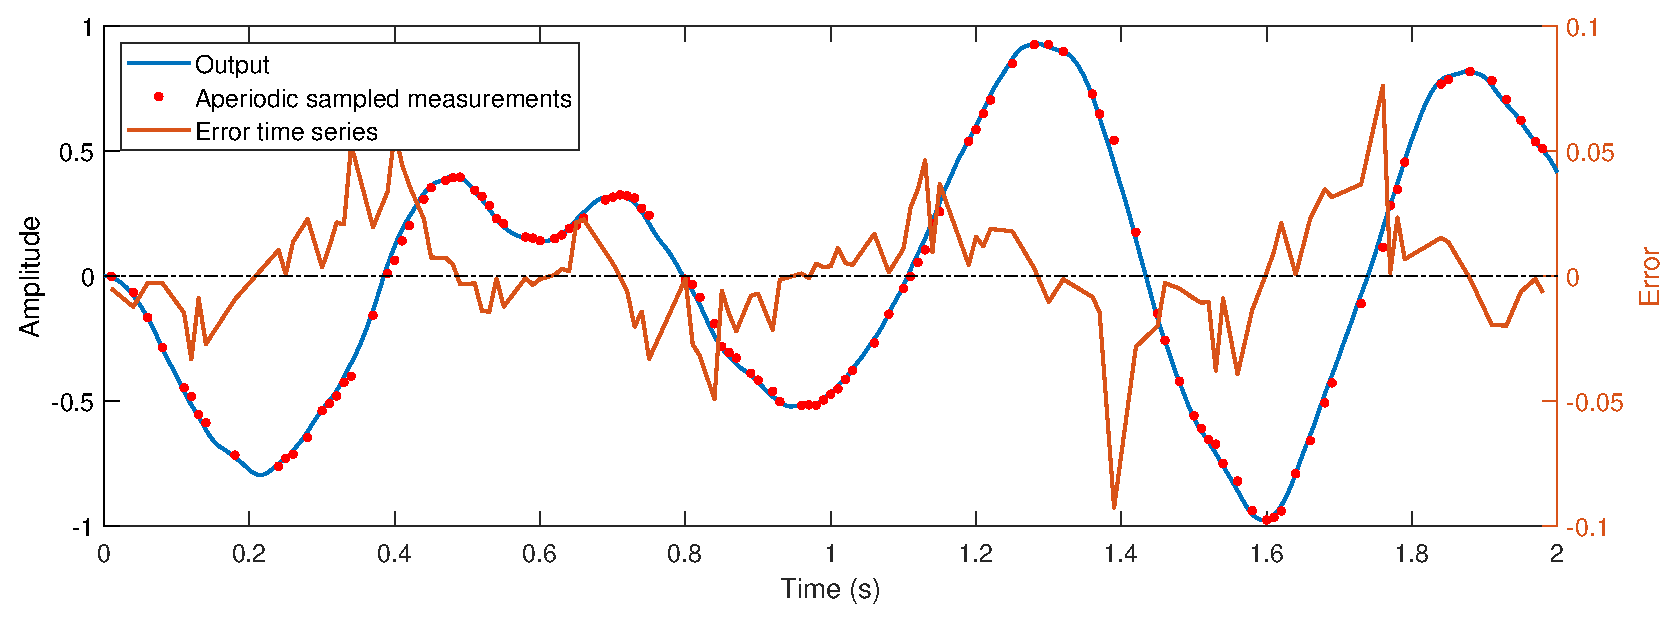
\includegraphics[width=0.75\textwidth]{Imagens/Gs_error.eps}
	\caption[Added error of shifting measurements time instants]{Added error time series (orange) as an effect of shifting time instants of the measurements (red) and output (blue). A gray dotted horizontal line is placed at the origin, for reference. Right scale (in orange) refers to the error data, whereas left scale (in black) refers to the output signal amplitude.}
	\label{fig:Gs_error}
\end{figure}

Additionally, the magnitude of the error is proportional to the opposite of the magnitude of the signal variation in the interval, that can be represented by its derivative. To better illustrate this aspect, we simulate new data, considering a much faster rate parameter of the Poisson process that generates the aperiodic sampling time instants, $\lambda=2$ kHz. The derivative of the signal is calculated, by multiplying $G(s)$ (\ref{eq:Gs_tf}) by $s$ and simulating the output of the resulting system for the same input sequence. Figure~\ref{fig:Gs_error_deriv} shows the original output, its derivative and the opposite of the error time series. We choose to plot the opposite of the error, to get a better grasp of how the magnitudes are related. In fact, we observe that the error values are directly proportional to the opposite of the signal derivative. Therefore, one conclusion we can draw is that the error cannot be modeled as a white Gaussian noise, since it has strong correlation with consecutive points. In fact, from the quantile-quantile plot \citep{Wilk1968} shown in Figure~\ref{fig:Gs_qq} we observe significant deviations from the quantiles of the error data in comparison to those from the theoretical normal distribution. That was expected, since the error is signal-dependent as shown in (\ref{eq:error_k}).

\begin{figure}[!htb]
	\centering
	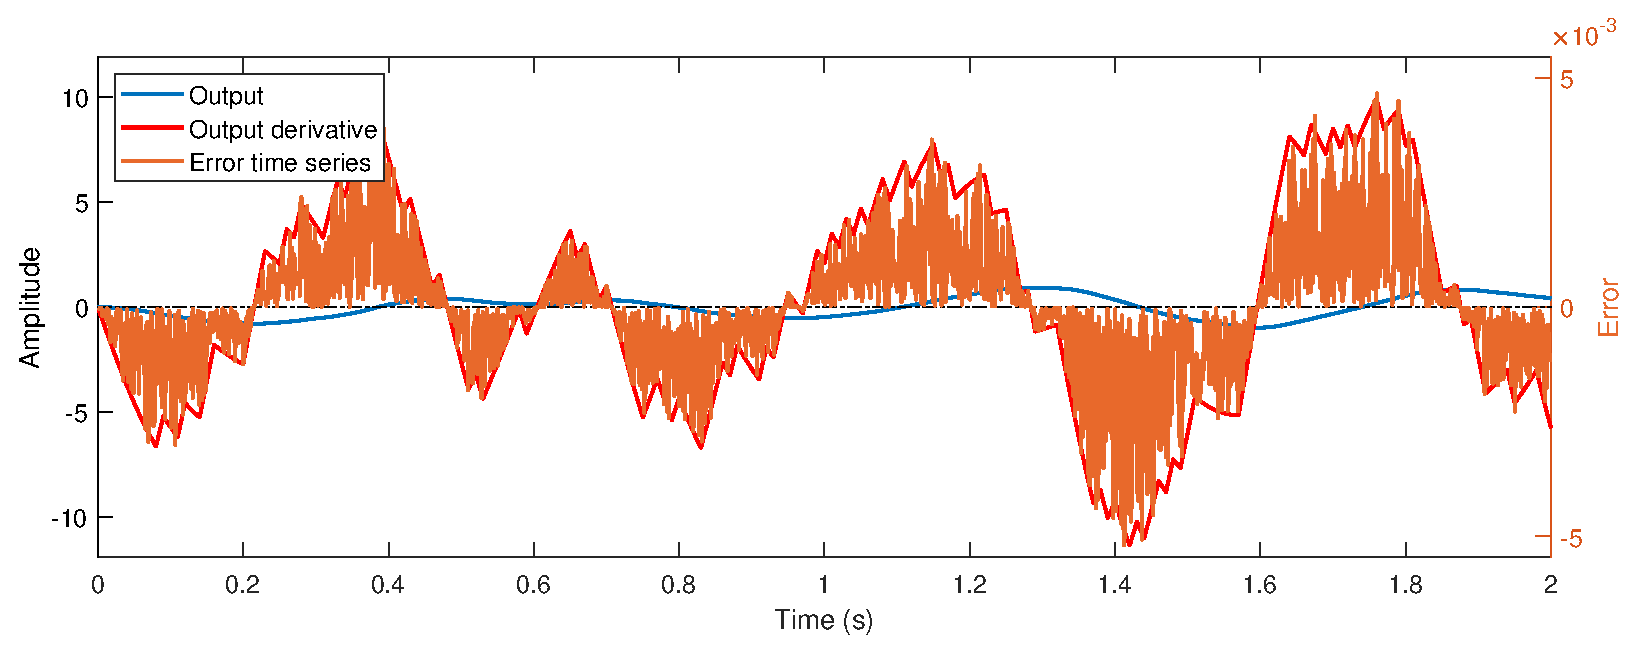
\includegraphics[width=0.75\textwidth]{Imagens/Gs_error_deriv.eps}
	\caption[Added error of shifting measurements time instants]{Opposite of the added error time series (orange) as an effect of shifting time instants of the measurements, output (blue) and its derivative (red). A gray dotted horizontal line is placed at the origin, for reference. We can see how the error is directly proportional to the opposite of the signal derivative.}
	\label{fig:Gs_error_deriv}
\end{figure}


\begin{figure}[!htb]
	\centering
	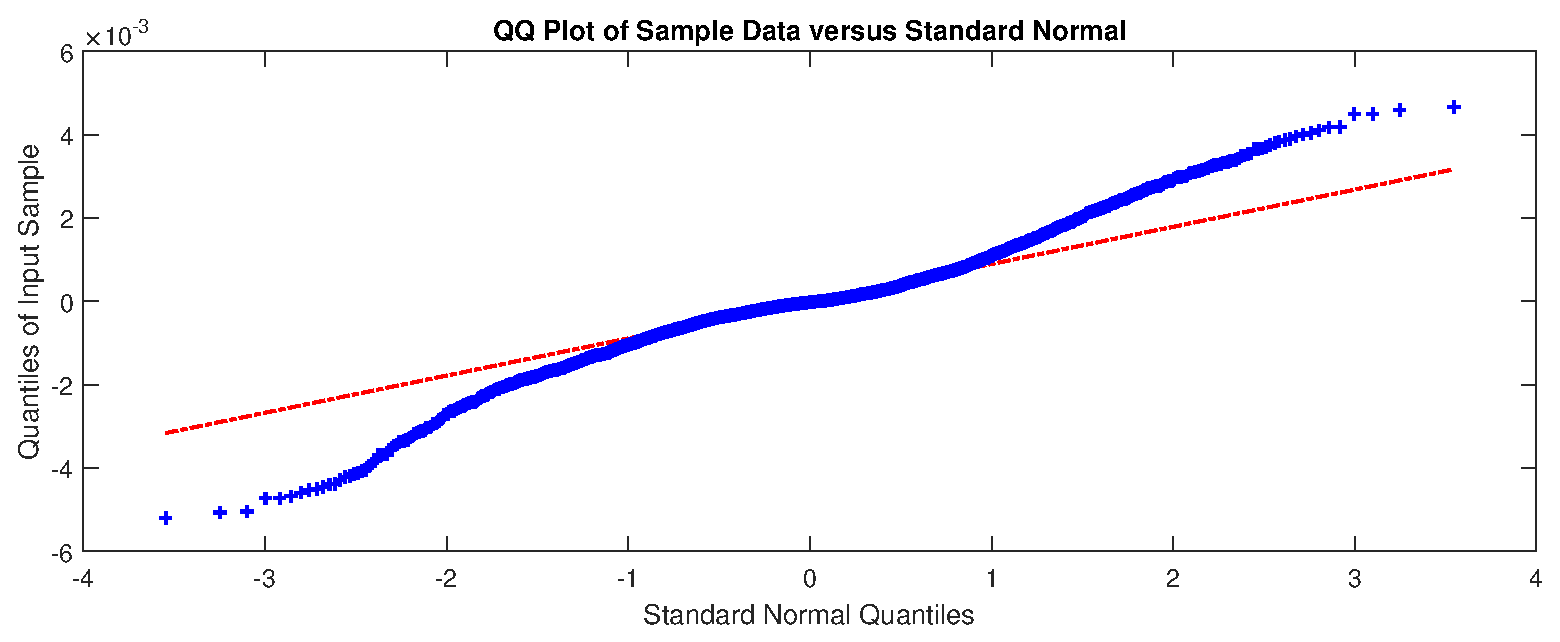
\includegraphics[width=0.75\textwidth]{Imagens/Gs_qq.eps}
	\caption[QQ-plot of the measurement error]{QQ-plot of the measurement error. Red line represents the expected quantiles of the standard normal distribution and the blue crosses, the error data quantiles.}
	\label{fig:Gs_qq}
\end{figure}

The simulated example did not consider any signal corruption from the measurements. In real applications, however, there will be additive sensor noise, usually modeled as white and Gaussian. Depending on their SNR values, the effect of the error $e$ might become irrelevant. To evaluate to what extent such claim is true, we carry out a 100-run simulation, varying both SNR and $\lambda$ values for the system from Example~\ref{ex:samp_error}. We estimate the RMSE contribution from $e$, by subtracting the total RMSE from the time-shifted measurements $\tilde{y}$ from measurements RMSE $y$ for each run. A surface plot of the results is shown in Figure~\ref{fig:surface}. We can see that both parameters affect the RMSE contribution from $e$. Higher SNR values and lower $\lambda$ are more sensible to the time shifting approximation for the signal. When measurement noise gets high enough, that is SNR lower than 60 dB, the RMSE contribution from $e$ is very close to zero. Similarly, if the average sampling rate of the measurements are faster than $5$ kHz, the noise levels are almost irrelevant, since the added RMSE is close to zero for all cases. These results motivate the design of different simulation scenarios for the state estimation problem.


\begin{figure}[!htb]
	\centering
	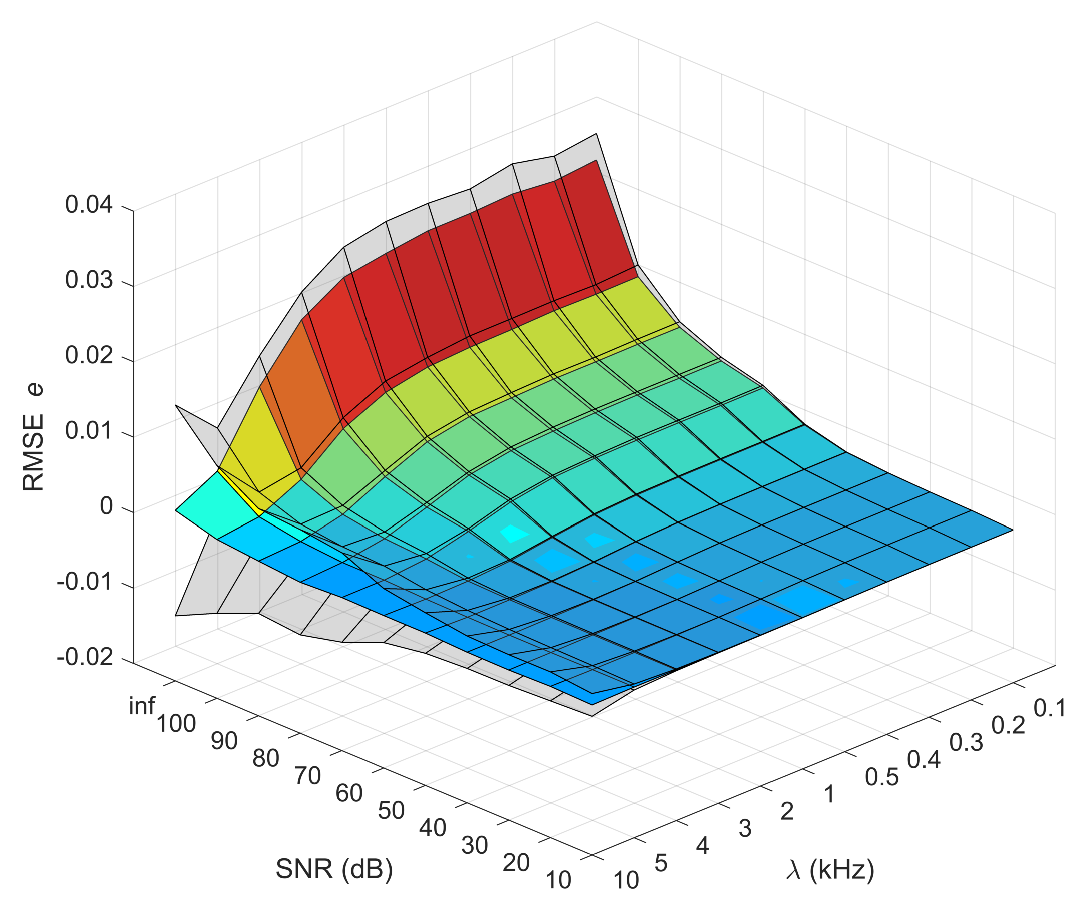
\includegraphics[width=0.75\textwidth]{Imagens/surface.eps}
	\caption[Surface plot of estimated RMSE from time shifting error, as a function of SNR and $\lambda$]{Surface plot of estimated RMSE from error $e$, as a function of SNR and $\lambda$. The transparent surfaces represent a confidence level of $95\%$.}
	\label{fig:surface}
\end{figure}


\section{Design of Simulation Setup}\label{sec:scenarios}

To evaluate performance and consistency effects of the aperiodic sampling in state estimation, we study three scenarios: (i) variation of noise level in signals, or SNR; (ii) variation of average measurement sampling rate $\lambda$; and (iii) variation of the relation between $\lambda$ and the regular estimation sampling rate $1/T$, that is $\alpha$. 

In the first scenario we intend to study how performance is affected by the presence of different noise levels in the signals. It is expected that the higher the noise, the closer will be the performance of both algorithms, as discussed in the previous section. The second scenario assesses how the average sampling rate of measurements $\lambda$, keeping $\alpha$ constant, is related to the degradation in performance when time-stamp is not considered in state estimation. Therefore, the speed of system dynamics in comparison to the sampling rate is investigated. In the last simulation scenario we study the behavior of the effects when the regular estimation frequency $1/T$ distances itself from the average observation sampling frequency $\lambda$. Additional errors due to measurement time instants approximation, as explained at the beginning of this chapter, are expected to have minor influence on the performance results.

Since estimation is performed in the presence of random quantities, we carry out several runs of simulations, so that confidence intervals can be constructed towards more consistent conclusions. We calculate average values from all runs with the corresponding $95\%$ confidence intervals for accuracy index $RMSE$, given by (\ref{eq:rmse}), and consistency tests $NEES$, given by (\ref{eq:nees}) and (\ref{eq:nees_h0}), and $NIS$, given by (\ref{eq:nis}) and (\ref{eq:nis_h0}). In Table~\ref{tab:symbols} we review some of the concepts and symbols that are extensively used in this chapter.


\begin{table}[!ht]
	\small
	\centering
	\setlength{\tabcolsep}{12pt}
	\caption[Review of concepts and symbols used in simulation]{Review of concepts and symbols used in the numerical results}
	\renewcommand{\arraystretch}{2}
	\begin{tabular}{S M L}	
		\toprule
		Symbol	& Definition  &  Description \\ 
		\midrule
		$\lambda$ (Section~\ref{sec:problem_form})		& $h_k \sim \mathcal{E} (\lambda)$ & Average sampling rate of observations, in Hz, determining random time intervals $h_k$   \\ 
		$T$	(Section~\ref{sec:problem_form})				& $t_i \triangleq iT$ & Regular estimation time interval, given in seconds \\ 
		$\alpha$ (Section~\ref{sec:problem_form})			& $\frac{1}{\lambda} \triangleq \alpha T$ & Relation between regular estimation time interval $T$ and average irregular time interval of observations $1/\lambda$   \\
		SNR (\ref{eq:snr_db}) 				& $SNR_{\textrm{dB}} \triangleq 10 \log_{10}\frac{P_{\textrm{signal}}}{P_{\textrm{noise}}}$ & Ratio between signal power $P_{\textrm{signal}}$ and noise power $P_{\textrm{noise}}$ in decibel, related to the level of data uncertainty \\
		NEES (\ref{eq:nees})			& $NEES \triangleq  \tilde{x}^T(P^{xx})^{-1}\tilde{x}$ & Value tested to be chi-squared distributed, in case of estimate error consistency \\
		NIS (\ref{eq:nis})					& $NIS \triangleq  \eta^T(P^{yy})^{-1}\eta$ & Value tested to be chi-squared distributed, in case of innovation consistency  \\ 
		
		$\mu_{\textrm{D}}$ (\ref{eq:ttest}) & $\mu_{\textrm{D}} \triangleq RMSE_\textrm{w/o} - RMSE_\textrm{w}$ & Mean difference of RMSE from algorithms considering and not considering timestamp \\
		
		Cohen's \textit{d} (\ref{eq:cohen}) & $d \triangleq \frac{\overline{RMSE}_\textrm{w/o} - \overline{RMSE}_\textrm{w}}{s_\textrm{D}}$ & Effect size estimate for the mean difference \\
		
		\bottomrule		
	\end{tabular}
	\label{tab:symbols}
\end{table}

\normalsize
\section{Linear System}

Our first system of choice is a fourth-order LTI system, since its results are more controllable and difference equations calculations have an exact solution. Thus results comparison and assessment are expected to be more easily grasped. Additionally, we choose the combination of two independent second order modes. One of the modes is a high-pass system with fast dynamics, and a the other a low-pass system with slower dynamics. The idea is to enable the evaluation of the effects in a separate way for different frequency responses. That is motivated by the fact that the error introduced by the measurements temporal shifts is directly related to the signal derivative, as shown in Section~\ref{sec:error_shift}.

\subsection{System Description}

The linear system chosen for simulation is the serial combination of two second order underdamped modes, with different band pass behaviors. Figure~\ref{fig:bode} shows the bode diagrams of both systems separately. One of the modes, henceforth termed as low-pass ($\textrm{lp}$) system, has a time constant $\tau_{\textrm{lp}} = 1$ s, a natural frequency $\omega_{n,\textrm{lp}} = 10$ Hz and a damping constant of $\zeta_{\textrm{lp}}=0.1$. The frequency response is then given by

\begin{equation}\label{eq:low-pass}
G_{\textrm{lp}}(s) = \frac{100}{s^2 + 2s + 100}.
\end{equation}

\noindent
The second mode is a high-pass ($\textrm{hp}$) system, with a lower time constant $\tau_{\textrm{hp}} = 0.01$ s, a higher natural frequency $\omega_{n,\textrm{hp}} = 1000$ Hz, and same damping constant of $\zeta_{\textrm{hp}}=0.1$, with two zeros, one at the origin and another one at $0.001$. The high-pass frequency response is given by:

\begin{equation}\label{eq:high-pass}
G_{\textrm{hp}}(s) = \frac{s^2-0.001s}{s^2 + 200s + 10^6}.\\
\end{equation}
\noindent

%\begin{figure}[!htb]
%	\centering
%	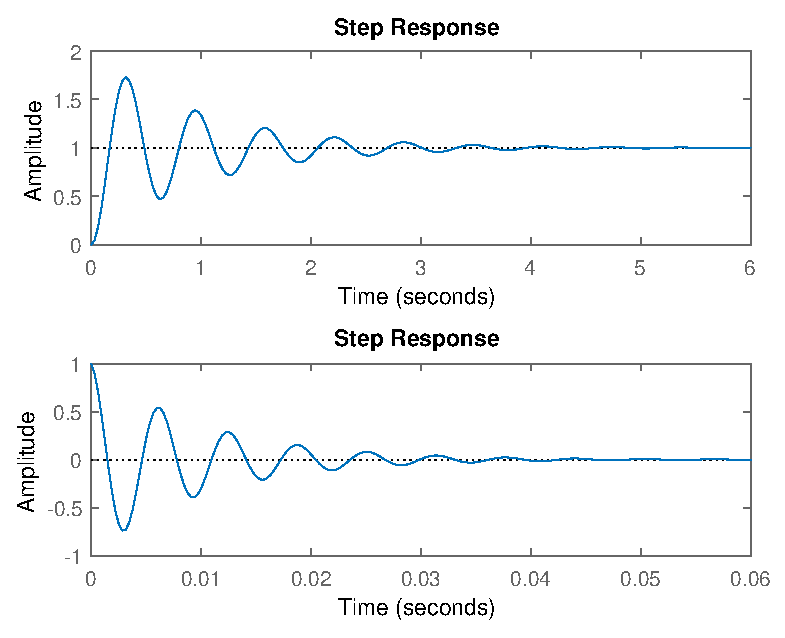
\includegraphics[width=0.6\textwidth]{Imagens/stepResponse.eps}
%	\caption[entrada]{Step response of both low-pass and high-pass modes.}
%	\label{fig:stepResponse}
%\end{figure}

\begin{figure}[!htb]
	\centering
	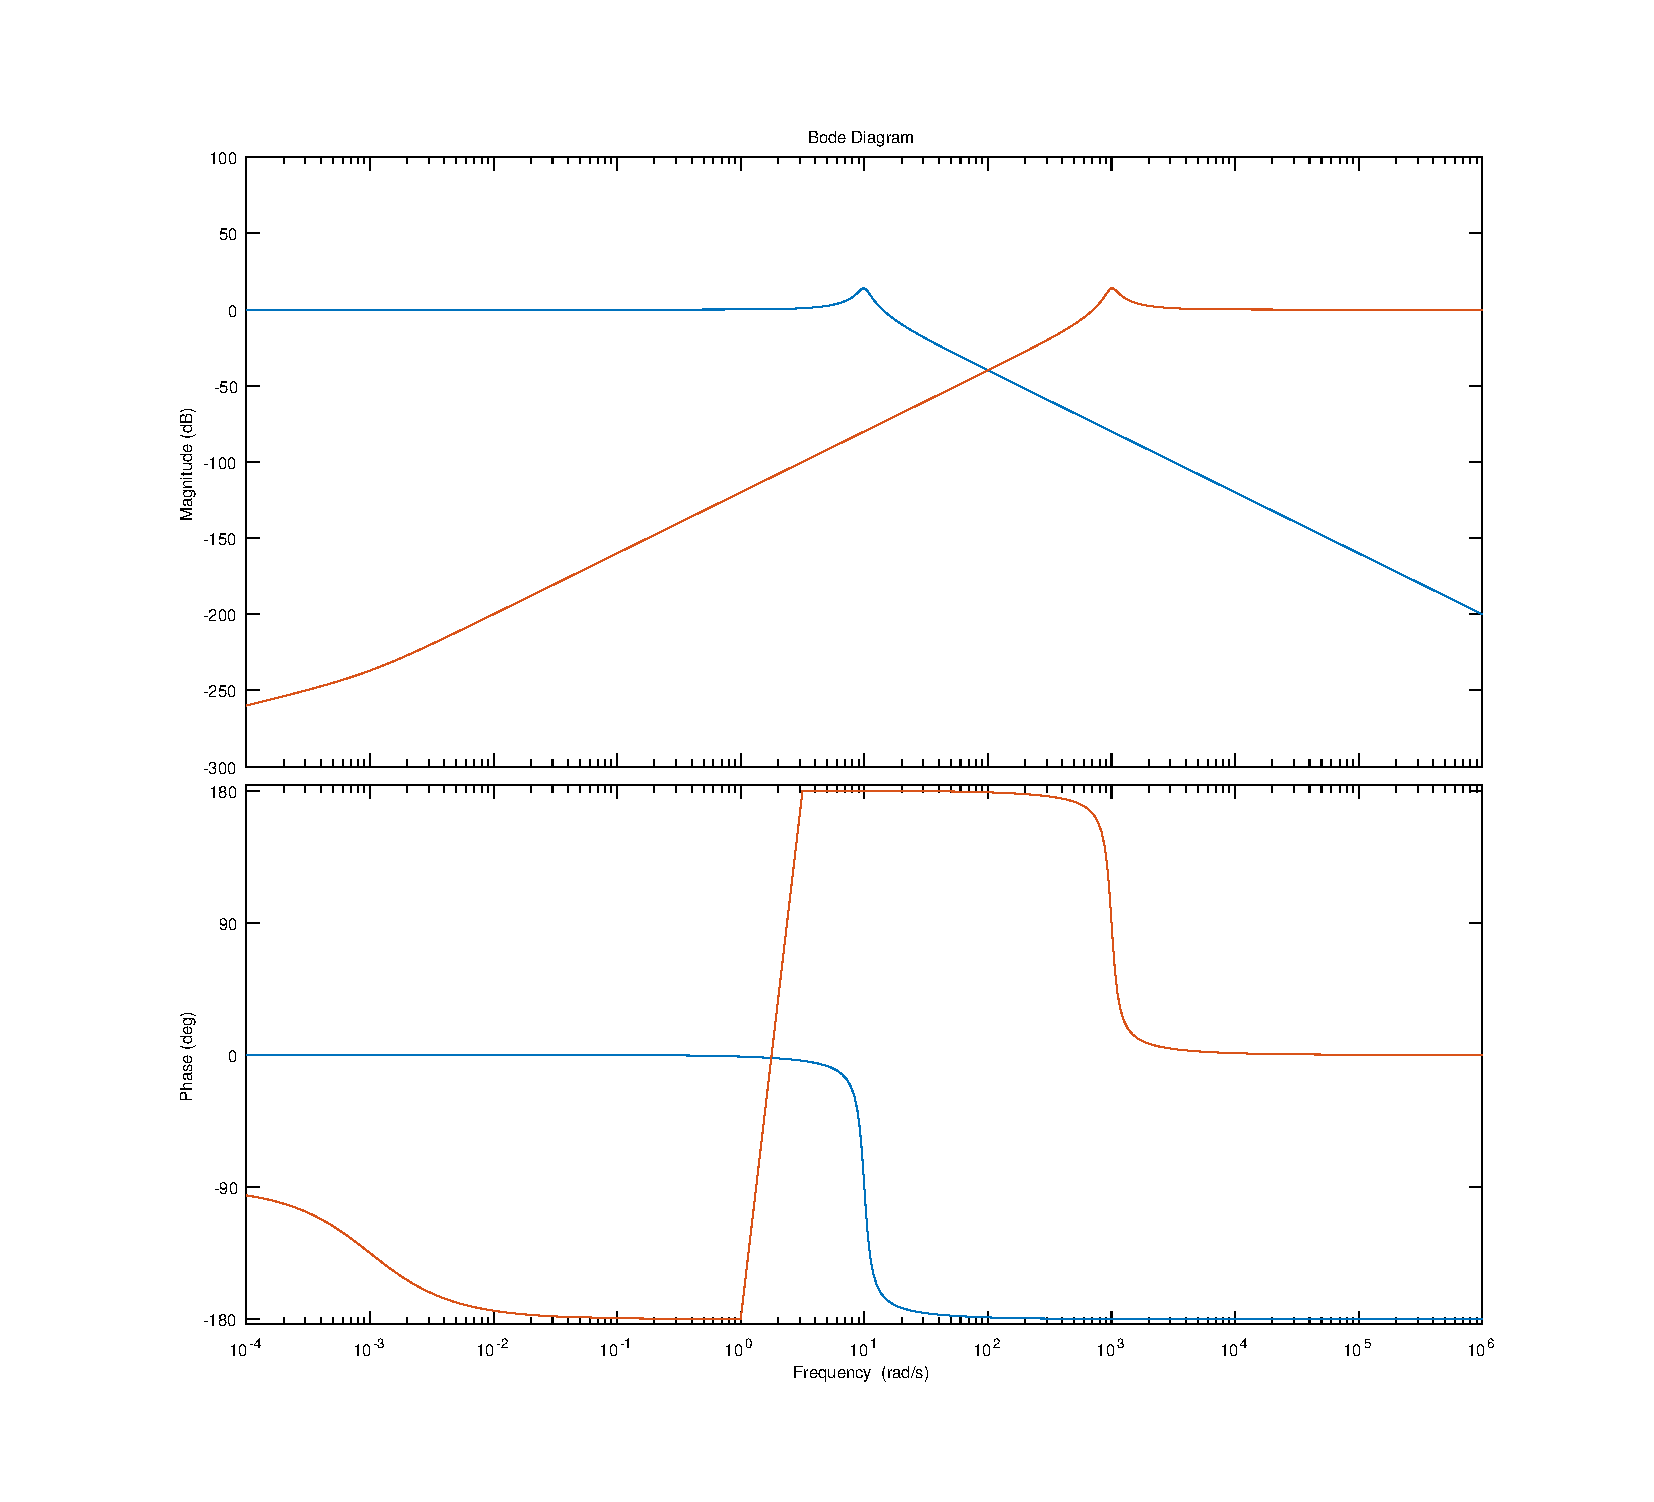
\includegraphics[width=0.5\textwidth]{Imagens/bode.eps}
	\caption[Bode diagram of both modes]{Bode diagram of both modes. Blue represent the low-pass system (\ref{eq:low-pass}) and red the high-pass system (\ref{eq:high-pass}).}
	\label{fig:bode}
\end{figure}

%\begin{figure}[!htb]
%	\centering
%	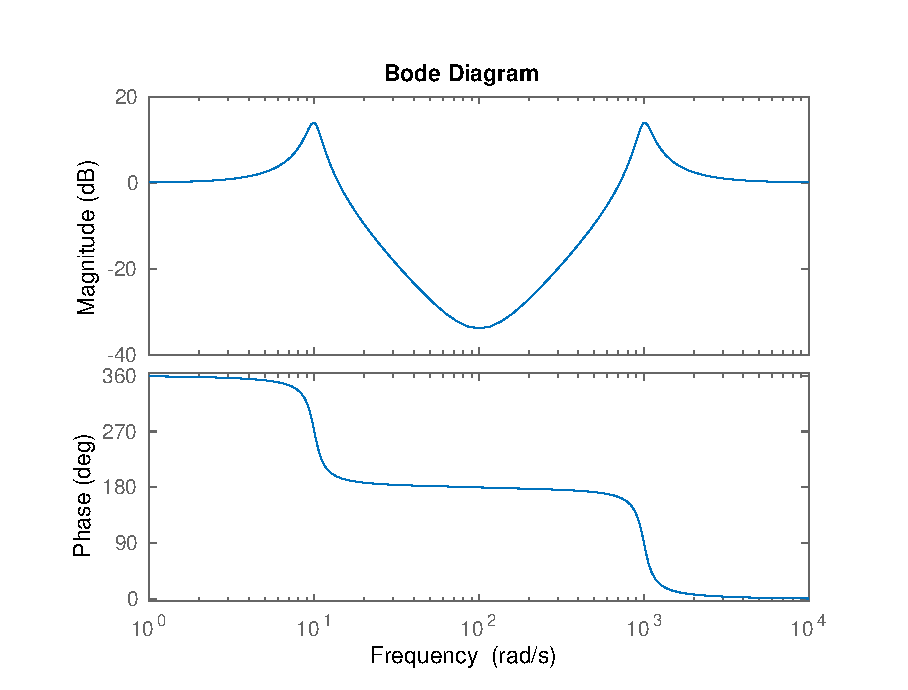
\includegraphics[width=0.6\textwidth]{Imagens/bodeS.eps}
%	\caption[entrada]{Bode diagram of the resulting fourth order system.}
%	\label{fig:bodeS}
%\end{figure}


The resulting fourth order system is described as a state space representation, in a modal canonical form given by:

\begin{align}
\dot{x}(t) & = Ax(t) + Bu(t) \label{eq:sys_beg}\\
y(t) & = Cx(t) + Du(t)
\end{align}


\noindent
where $x(t) \in \mathbb{R}^4$ is the state vector, $u(t) \in \mathbb{R}^1$ is the single input vector and $y(t) \in \mathbb{R}^1$ is the single output vector, and

\begin{align}
A & =\begin{bmatrix}
-100 & 994.99 & 0 & 0\\
-994.99 & -100 & 0 & 0\\
0 & 0 & -1 & 9.949\\
0 & 0 & -9.949 & -1
\end{bmatrix}, \label{eq:linear_A}\\
B & =\begin{bmatrix}
-24.6435 \\
-18.8943 \\
-4.1746 \\
-0.2675
\end{bmatrix}, \\
C & =\begin{bmatrix}
24.41 & -21.2522 & -0.1537 & 2.3977 \\
\end{bmatrix}, \\
D & =1. \label{eq:sys_end}
\end{align}

\noindent
Matrix $A$, given by (\ref{eq:linear_A}), indicates two subsystem dynamically decoupled. The upper diagonal block refers to the high-pass system (\ref{eq:high-pass}), whereas the lower diagonal block represents the low-pass system (\ref{eq:low-pass}).

%
%\begin{equation}\label{eq:sistemaLinear}
%\begin{split}
%Z_{de} & := (\partial Z/\partial \delta_e)/m = -61.655 \ m/s^2,\\
%Z_q & := (\partial Z/\partial q)/m = -5.132 \ m/s,\\
%Z_w & := (\partial Z/\partial W)/m = -3.1332 \ s^{-1},\\
%M_{de} & := (\partial M/\partial \delta_e)/I_y = -40.465 \ s^{-2},\\
%M_q & := (\partial M/\partial q)/I_y = -2.6864 \ s^{-1},\\
%M_w & := (\partial M/\partial W)/I_y = -0.04688 \ (s-m)^{-1},\\
%\tau & = 0.1 \ s \\
%U_o & = 306.42 \ m/s
%\end{split}
%\end{equation}

We simulate a pseudo-random binary sequence (PRBS) as input, with 200 samples, as shown in Figure~\ref{fig:prbs}. The PRBS signal is used as input to the low-pass and high-pass systems separately, considering two different time frames, of 2 and 20 seconds. The results of the four linear simulations are shown in Figure~\ref{fig:sys_results}. The 20 seconds simulation for the high-pass system achieve steady state values very quickly, such that it is not easy to observe the influence of the system dynamics on the results. Thus, we choose the 2 seconds time frame to simulate the fourth order serialized systems, given by (\ref{eq:sys_beg})-(\ref{eq:sys_end}). The result of the linear simulation of the fourth order system is presented in Figure~\ref{fig:4ordersys2s}.


\begin{figure}[!htb]
	\centering
	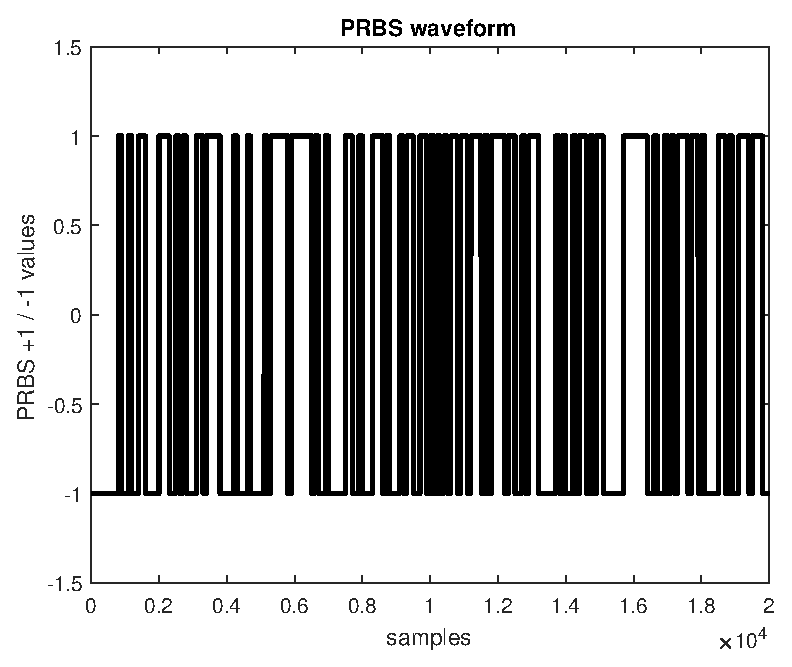
\includegraphics[width=0.75\textwidth]{Imagens/prbs.eps}
	\caption[PRBS samples used as input]{200 PRBS samples used as input to simulate system (\ref{eq:sys_beg})-(\ref{eq:sys_end})}
	\label{fig:prbs}
\end{figure}

\begin{figure}[!htb]
 	\centering
 	\subfigure[]{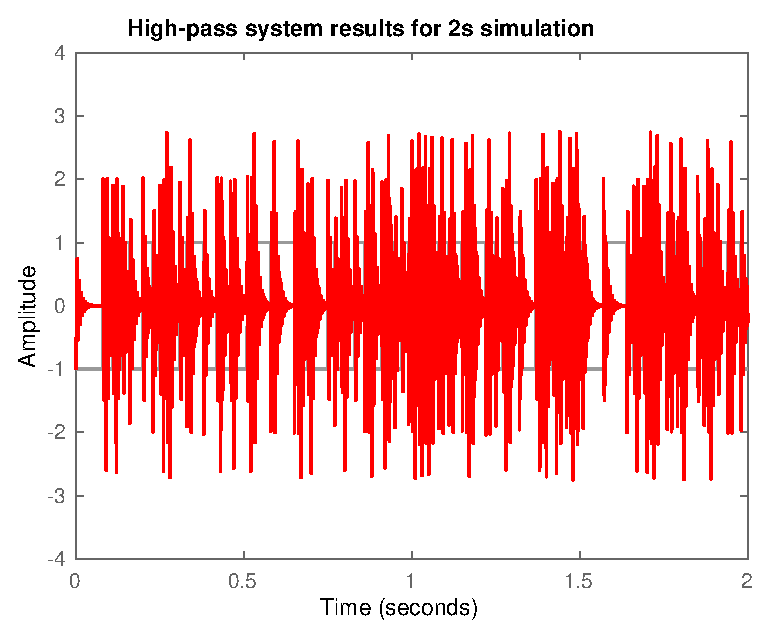
\includegraphics[width=0.45\textwidth]{Imagens/hp2s.eps}}
 	\subfigure[]{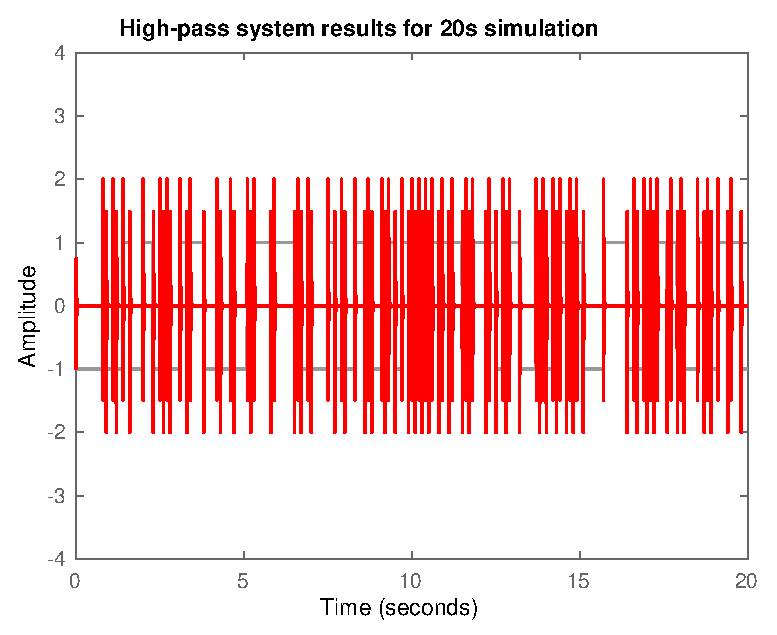
\includegraphics[width=0.45\textwidth]{Imagens/hp20s.eps}} \\
 	\subfigure[]{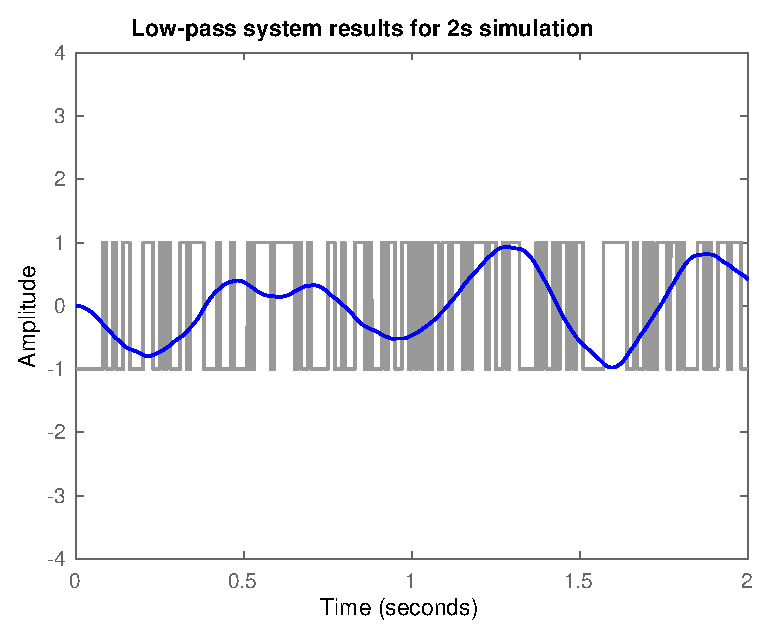
\includegraphics[width=0.45\textwidth]{Imagens/lp2s.eps}} 
 	\subfigure[]{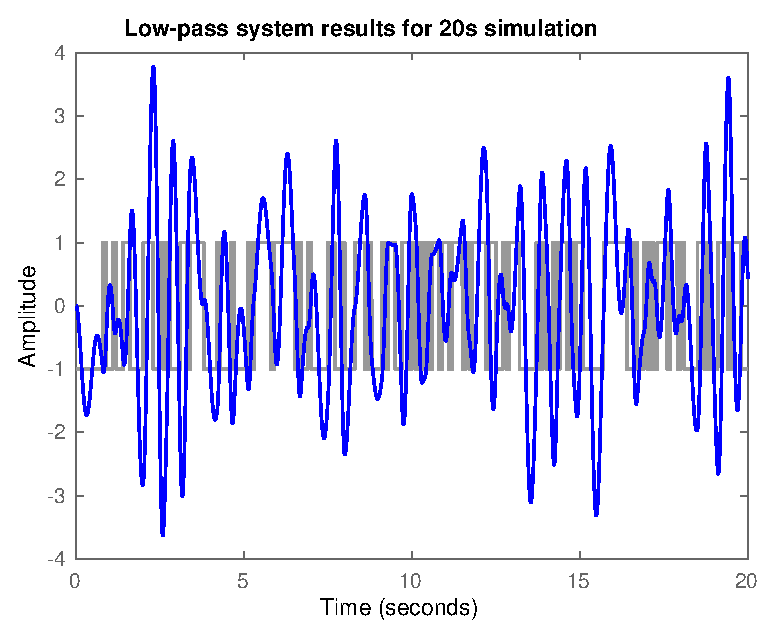
\includegraphics[width=0.45\textwidth]{Imagens/lp20s.eps}}
 	\caption[Linear simulation results for PRBS input in different time frames]{Linear simulation results of the low-pass and high-pass systems separately. Grey lines represent the PRBS input and colored lines the output. Graphs (a) and (b) with red outputs represent the results of the high-pass system; and (c) and (d) with blue outputs, the results of the low-pass system. Graphs on the left show a time frame of 2 seconds of simulations, whereas the ones on the right are the result of a 20 seconds time frame; considering the same 200 samples of PRBS for all four simulations.} 
 	\label{fig:sys_results}
 \end{figure}


\begin{figure}[!htb]
	\centering
	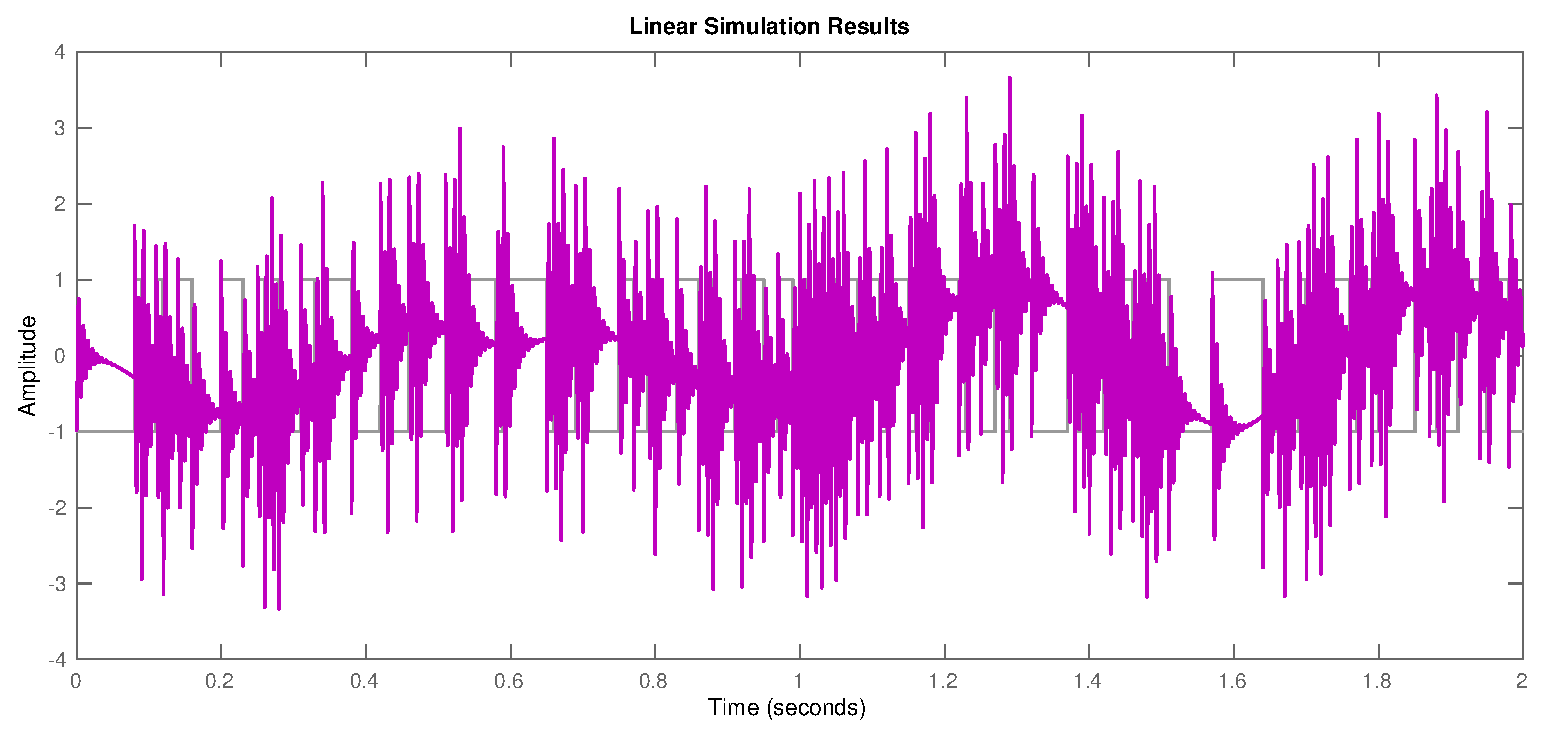
\includegraphics[width=0.8\textwidth]{Imagens/4ordersys2s.eps}
	\caption[Output of the fourth order system to the PRBS input signal]{Output of the fourth order system to the PRBS input signal over a 2 seconds time frame.}
	\label{fig:4ordersys2s}
\end{figure}

System discretization is performed using exact discretization for inputs considered constant during each time interval to produce a discrete-time state space representation according to

\begin{align}
x(t_{k+1}) &= A_{\textrm{d}}(t_k) x(t_k) + B_{\textrm{d}} u(t_k) + w(t_k), \\
y(t_k) &= B_{\textrm{d}}x(t)+D_{\textrm{d}}u(t) + v(t_k)
\end{align}

\noindent
where $t_{k+1} = t_k + h_k \in \mathbb{R}$ and $k \in \mathbb{N}$. $\rho(v(t_k)) = \mathcal{N} (0,R)$ and $\rho(w(t_k)) = \mathcal{N} (0,Q)$ are, respectively, the process and observation noise, with zero mean and covariance $R$ and $Q$. When timestamp is not available, the observation vector is approximated by $\tilde{y}_i \approx y(t_k)$, where $i$ is the index of the next regular estimation time instant, multiple of $T$. When it is available, discretization is performed using variable time intervals.

\subsection{Single Realization Analysis}

In this section we present one realization of the state estimation simulation for the system defined by (\ref{eq:sys_beg})-(\ref{eq:sys_end}), using the Kalman Filter described in Section~\ref{sec:kalman-filter} and the algorithm modifications explained in Section~\ref{sec:estimation_aperiodic}.  

Simulation parameters are set according to $\lambda = 500 \textrm{ Hz}$, $SNR_{\textrm{obs}} = 30 \textrm{ dB}$, and $SNR_{\textrm{pro}} = 30 \textrm{ dB}$, where subscript $\textrm{obs}$ and $\textrm{pro}$ refer to observation and process, respectively. Time step to simulate nominal system model is set as $\delta t_{\textrm{sim}} = 10^{-6} \textrm{ s}$ and the regular estimation time interval is given by $T = 2\times 10^{-3} \textrm{ s}$. Noise is generated as a zero mean, white, Gaussian signal with $R=9.596\times 10^{-4}$ and process noise variance of $Q=9.986\times 10^{-4}I_{4\times 4}$. These exact values are used in the Kalman filter implementation and the estimation results for states $x_1$ and $x_4$ of the algorithms with and without timestamp, in comparison to the true state values are shown in Figures~\ref{fig:StatesWithAndWithoutTimeStamp}.

\begin{figure}[!htb]
	\centering
	\subfigure{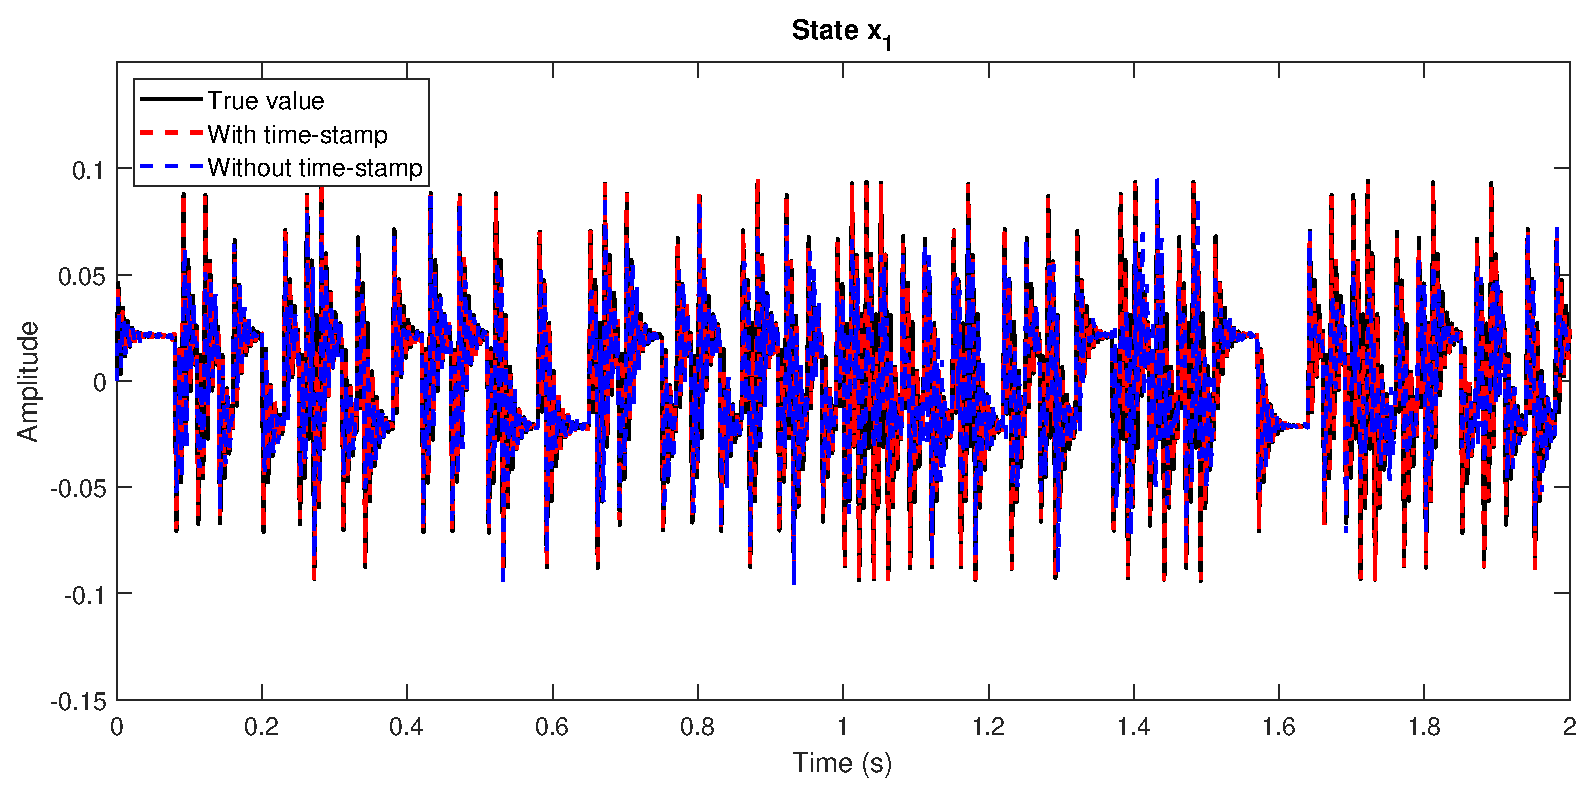
\includegraphics[width=0.75\textwidth]{Imagens/StatesWithTimeStamp.eps}} \\
	\subfigure{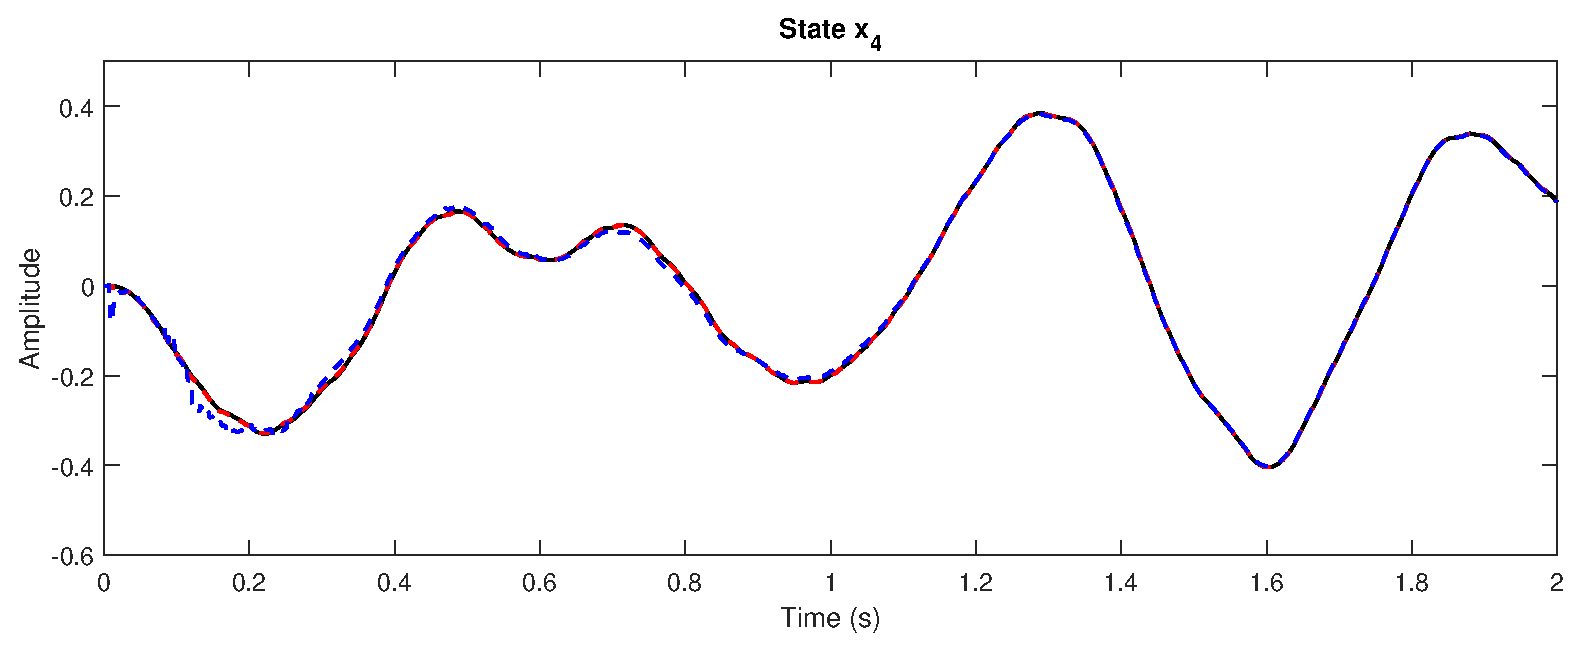
\includegraphics[width=0.75\textwidth]{Imagens/StatesWithoutTimeStamp.eps}}  
	\caption[Estimated and true states]{States $x_1$ (high-pass) and $x_4$ (low-pass) estimates with timestamp (\textcolor{red}{- -}), without timestamp (\textcolor{blue}{- -}) and true values (\textcolor{black}{---}).}
	\label{fig:StatesWithAndWithoutTimeStamp}
\end{figure}

For both systems states, we observe the degradation for the algorithm that approximates time instants $t_k$ in the estimation process, represented by the dashed blue lines.


Figure~\ref{fig:LinearJevolution} presents a data window from 0 to 0.013 seconds of the accuracy index RMSE of state $x_2$, for the algorithms with and without timestamp. As expected, when first observation arrives, RMSE results distance themselves, in favor of the algorithm that considers timestamp. The RMSE difference increases when the next measurement (the second one) arrives. For the time period without observations, indexes of both algorithms evolve in a similar way. 
 	
\begin{figure}[!htb]
	\centering
	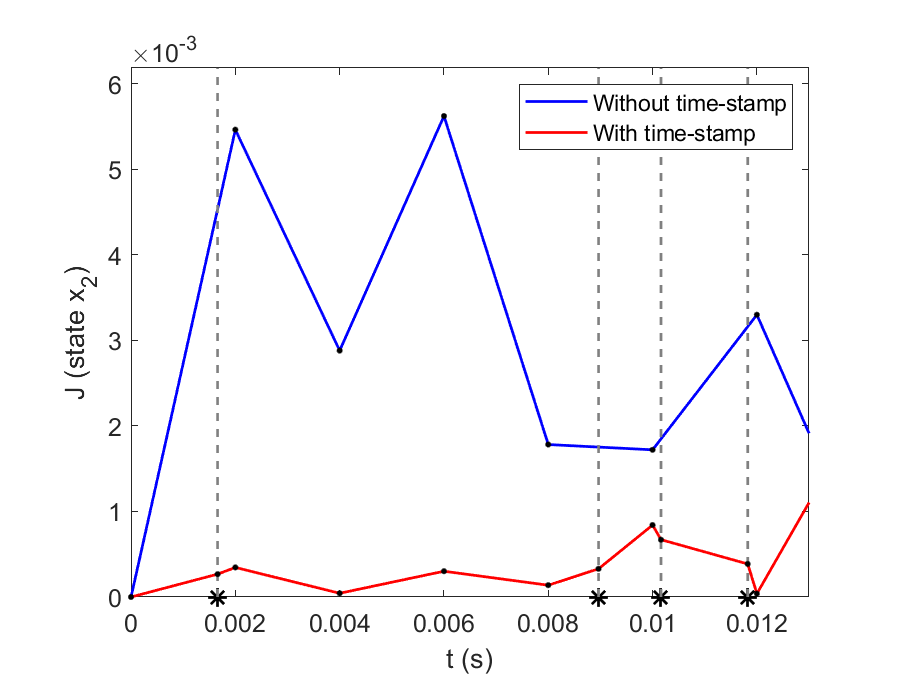
\includegraphics[width=0.6\textwidth]{Imagens/LinearJEvolution.eps}
	\caption[Performance index temporal cut for one realization]{Temporal cut from 0 to 0.013 seconds, for a realization of state $x_2$ RMSE for	 both estimators, with (\textcolor{red}{---}) and without (\textcolor{blue}{---}) timestamp. Vertical dashed lines match the measurement sampling instants $t_k$. Black dots represent the estimation instants.}
	\label{fig:LinearJevolution}
\end{figure}

Finally, for this realization, we also present single-run consistency tests, using the indices NEES and NIS, as defined in Section~\ref{sec:metrics}, in Figure~\ref{fig:linearConsistency}. In each graph, the acceptance intervals are marked by horizontal lines. The upper plots (a) and (b) represent the NEES and NIS values, respectively, for the algorithm that considers timestamp in the estimation process. We can see that the estimates are quite consistent, with the values inside the acceptance region most of the time. In fact, the null hypothesis rejection rate, that is the proportion of times the values were out of their acceptance region, was $4\%$ for NEES, and $5,5\%$ for NIS, very close the the $5\%$ expected. When timestamp was not available, consistency was heavily degraded, with rejection rates escalating to $61\%$ and $43\%$, respectively. Moreover, NEES and NIS values were so high in some occasions, that the acceptance region is hardly visible in the graphs. In practice, such a consistency degradation means that estimation covariances are highly underestimated.

 \begin{figure}[!htb]
	\centering
	\subfigure[]{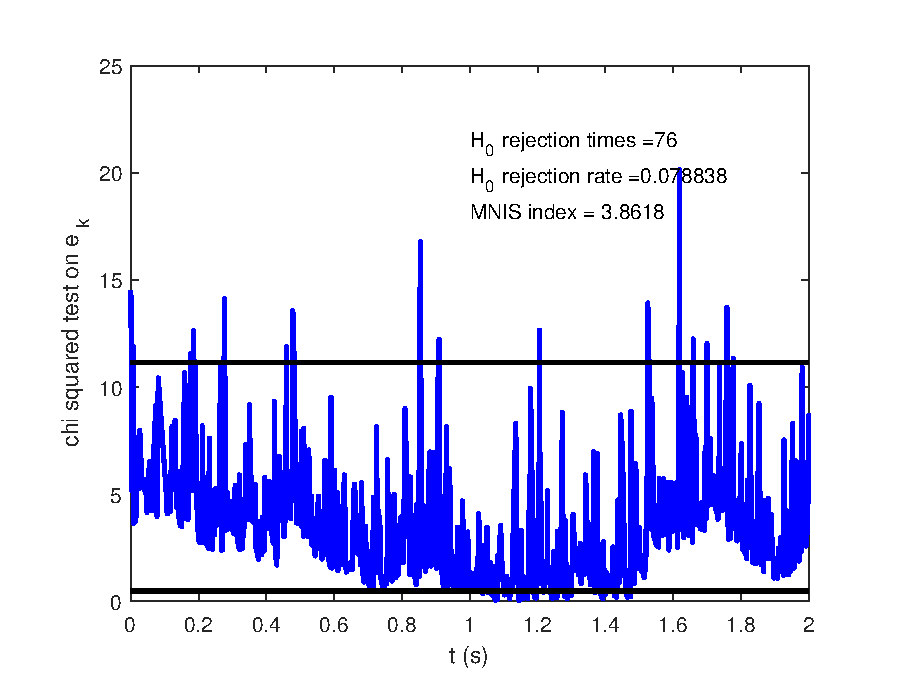
\includegraphics[width=0.45\textwidth]{Imagens/chi_e_with.eps}} 
	\subfigure[]{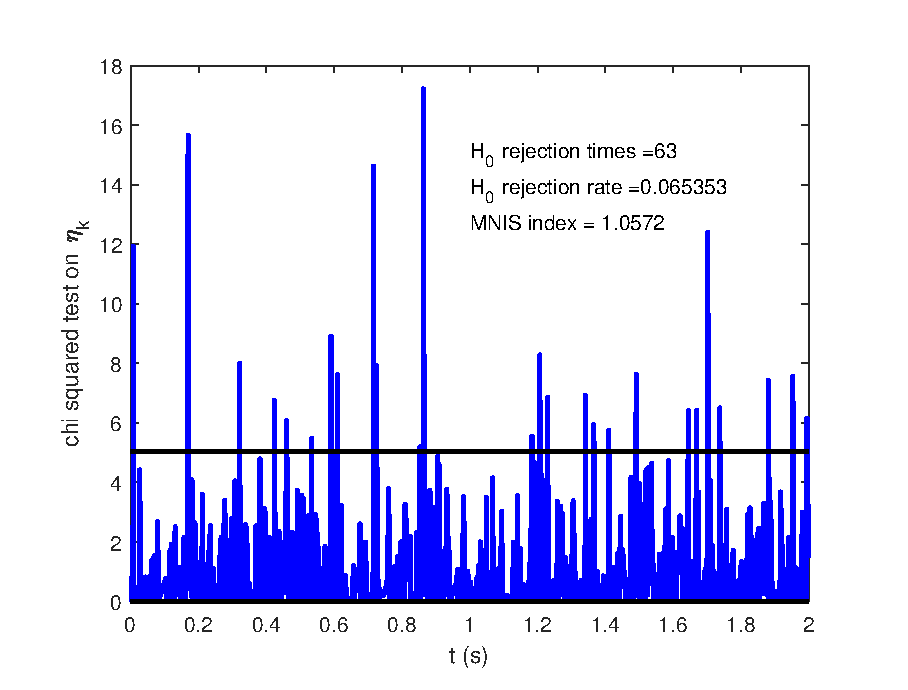
\includegraphics[width=0.45\textwidth]{Imagens/chi_eta_with.eps}}  \\
	\subfigure[]{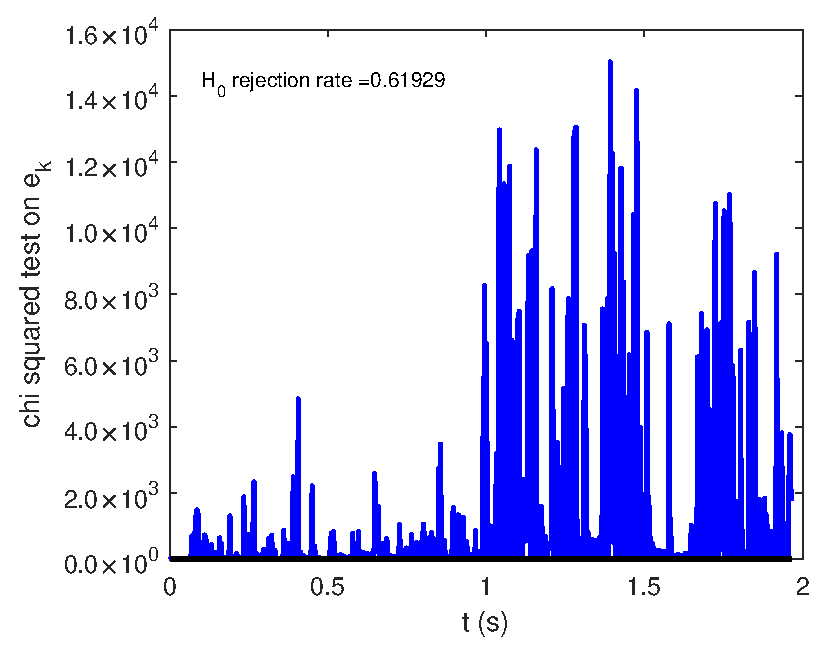
\includegraphics[width=0.45\textwidth]{Imagens/chi_e_without.eps}}
	\subfigure[]{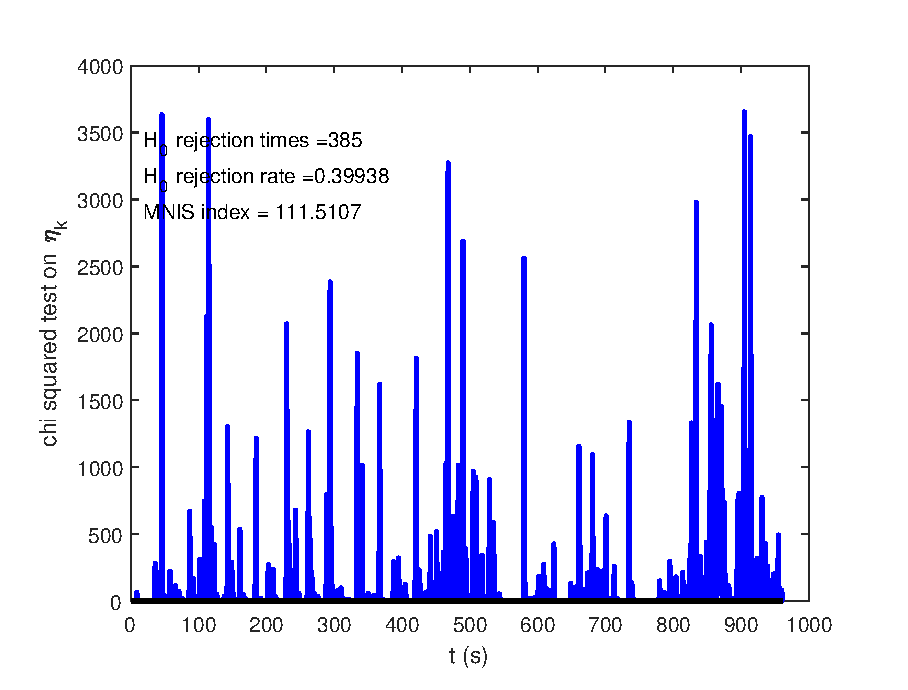
\includegraphics[width=0.45\textwidth]{Imagens/chi_eta_without.eps}}
	\caption[Consistency tests for linear system]{Consistency tests NEEs and NIS for the linear system state estimation with timestamps (a) and (b); and without timestamp (c) and (d). Horizontal lines define the acceptance region upper and lower limits, for a significance level $\alpha=0.05$. In each graph, the null hypothesis $H_0$ rejection rate is also presented.}
	\label{fig:linearConsistency}
\end{figure}

In the next sections we study the scenarios described in Section~\ref{sec:scenarios} for multiple runs. The simulation parameters are defined according to Table~\ref{tab:params_linear} and a 100-run Monte Carlo simulation is performed for each of the parameter set. Only the results of one state per mode are shown, namely $x_1$ and $x_4$, for simplicity sake. We present the paired t-test results for states $x_1$ and $x_2$ in Table~\ref{tab:results_linear}. Figure~\ref{fig:linear_sim} encompasses all performance metrics results for all scenarios. Each column contains the performance metrics variation for each scenario.

\begin{table}[!ht]
	\centering
	\setlength{\tabcolsep}{12pt}	
	\caption[Sets of parameters for linear system simulation]{Sets of parameters for linear system simulation}
	\renewcommand{\arraystretch}{1.5}
	\small
	\begin{tabular}{c | c | c | c }
		\toprule
		Scenario & SNR (dB)	& $\lambda$ (Hz) & $\alpha$\\
		\midrule
		SNR variation & $[60,\ 50,\ 40,\ 20,\ 10]$	& $500$ & $1$ \\ 
		$\lambda$ variation & $30$		&  $[1000,\ 500,\ 200,\ 100]$ & $1$  \\ 
		$\alpha$ variation & $30$		&  $500$ & $[5,\ 3,\ 2,\ 1]$  \\ 
		\bottomrule
	\end{tabular}
	\label{tab:params_linear}
\end{table}

\subsection{Measurement Signal-to-Noise Ratio Variation}\label{sec:ruido-AC}

%For the first simulation scenario, we consider SNR variation for both the process and observation models jointly. Chosen parameters are presented in Table~\ref{tab:params_linear_snr} and results for the performance metrics are shown in column (a) of Figure~\ref{fig:linear_sim}.


%\begin{table}[!ht]
%	\centering
%	\setlength{\tabcolsep}{12pt}
%	\caption[Linear system simulation parameters for SNR variation]{Linear system simulation parameters for SNR variation}
%	\begin{tabular}{c | c | c }
%		\toprule
%		SNR (dB)	& $\lambda$ (Hz) & $\alpha$\\
%		\midrule
%		$[60,\ 50,\ 40,\ 20,\ 10]$	& $500$ & $1$ \\
%		\bottomrule
%	\end{tabular}
%	\label{tab:params_linear_snr}
%\end{table}

%Regular estimation time interval $T$ is maintained fixed at $T=0.002 \textrm{s}$  and $\alpha=1$, thus $\lambda=500 \textrm{Hz}$. For a 100-run simulation, the obtained results for accuracy and consistency are presented in Figure~\ref{fig:linearNoise} with the corresponding $95\%$ confidence intervals.


% \begin{figure}[!htb]
%	\centering
%	\subfigure[]{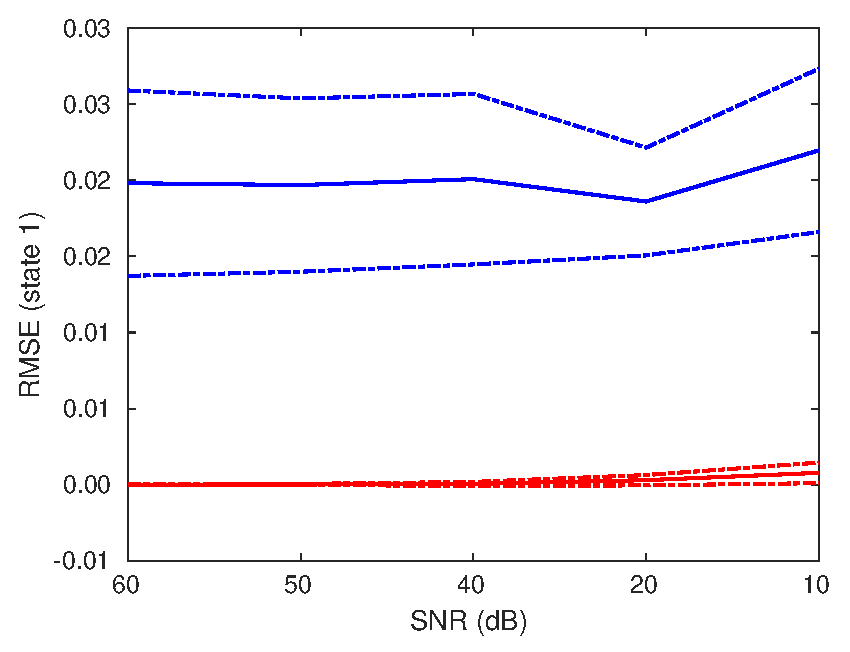
\includegraphics[width=0.49\textwidth]{Imagens/linearNoise_x1_rmse.eps}} 
%	\subfigure[]{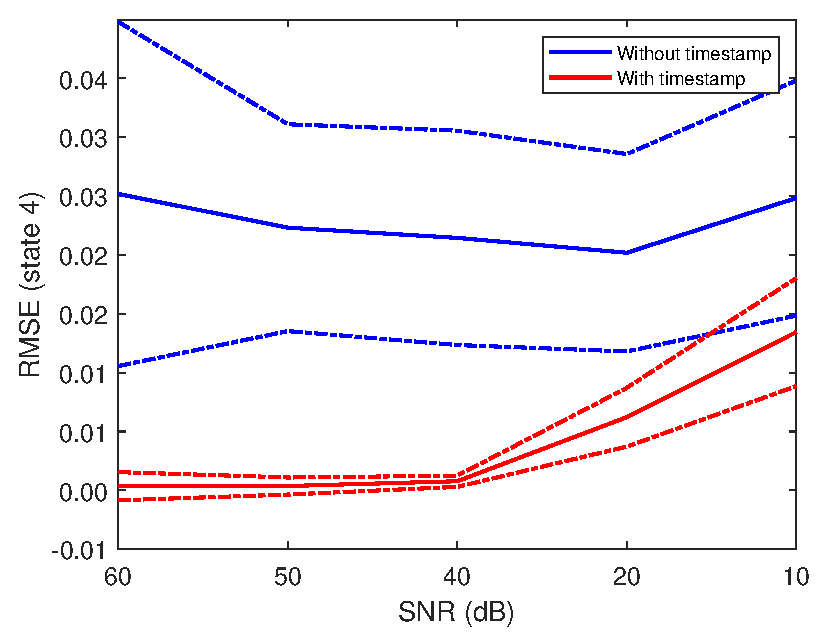
\includegraphics[width=0.49\textwidth]{Imagens/linearNoise_x4_rmse.eps}}  \\
%	\subfigure[]{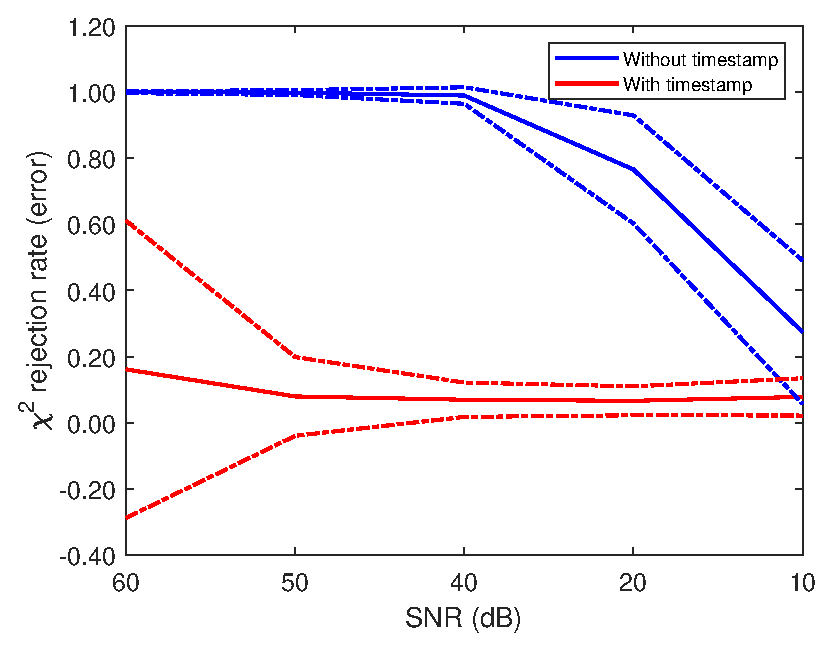
\includegraphics[width=0.49\textwidth]{Imagens/linearNoise_NEES.eps}}
%	\subfigure[]{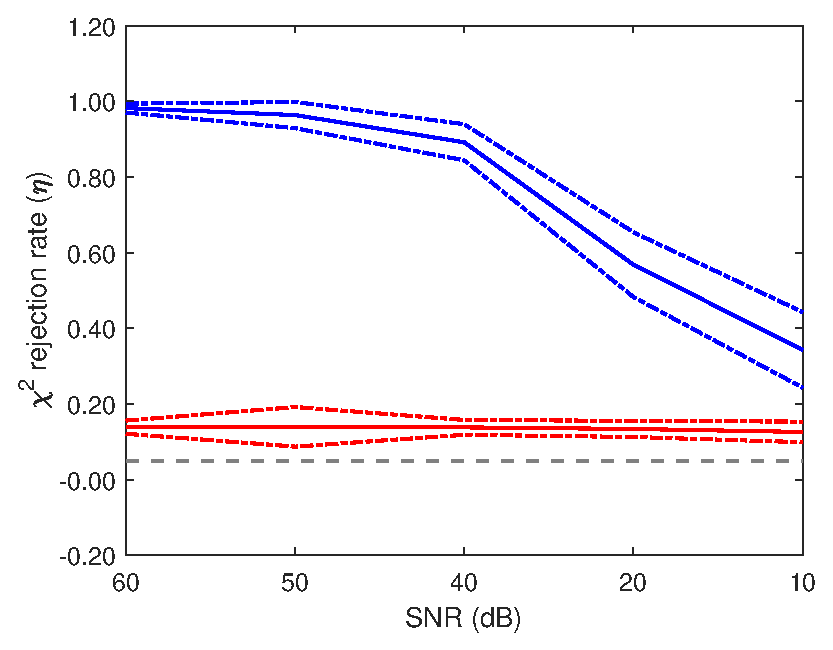
\includegraphics[width=0.49\textwidth]{Imagens/linearNoise_NIS.eps}}
%	\caption[Linear system estimation performance, as a function of input and observation SNR]{Linear system estimation performance indices with $95\%$ confidence intervals, as a function of input and observation SNR, for algorithms with (\textcolor{red}{---}) and without (\textcolor{blue}{---}) time-stamp. Accuracy values for states $x_1$ and $x_2$ are shown in (a) and (b), respectively. Consistency results are in (c) and (d) for NEES and NIS tests, respectively.}
%	\label{fig:linearNoise}
%\end{figure}


Results from the first row of Table~\ref{tab:results_linear} suggest an increasing trend of RMSE degradation as we increase SNR levels, with an apparent upper bound limit. The mean differences of both states $x_1$ and $x_4$ have no significant variation for SNR levels as high as 40, 50 and 60 dB. On the other hand, when noise level is high, with SNR$=10$ dB, the RMSE differences have much smaller practical significance, with an effect size of approximately $0.7$ standard deviation for both states.

In the first column of Figure~\ref{fig:linear_sim} we can observe a decreasing monotonic behavior for RMSE results of the algorithm considering timestamp, as SNR levels increase, as expected. However, the same behavior cannot be observed for the method that neglects timestamp information. In fact, RMSE results for state $x_4$ reduce for higher noise levels in data. Such trend can be explained by the fact that, for higher SNR, the added error introduced by shifting time instants plays a more important role in the degradation of the estimates. When SNR decreases, its relevance is reduced, and the covariance matrix used by the algorithms are closer to the reality. Thus estimates are more consistent and for the low-pass system state $x_4$ results have lower RMSE.

As for NEES and NIS tests, considering timestamp produces consistent estimates for all cases, with mean rates for NEES and NIS near the $5\%$ significance level. On the other hand, not considering timestamps produced inconsistent results in all scenarios, specially when there are lower noise levels in the data.

Finally, the shapes of the box and whiskers plots suggest a sample distribution with higher variability for accuracy results of the algorithm that neglects timestamp, which means less reliability in the estimation.

\subsection{Average Sampling Rate Variation}\label{sec:lambda-AC}

%In the second simulation scenario for the linear system, we consider a variation of average sampling rate of observation $\lambda$, keeping other parameters fixed. Table~\ref{tab:params_linear_lambda} shows the used parameters and column (b) of Figure~\ref{fig:linear_sim}, the obtained results.

%
%\begin{table}[!ht]
%	\centering
%	\setlength{\tabcolsep}{12pt}
%	\caption[Linear system simulation parameters for $\lambda$ variation]{Linear system simulation parameters for $\lambda$ variation}
%	\begin{tabular}{c | c | c }
%		\toprule
%		SNR (dB)	& $\lambda$ (Hz) & $\alpha$ \\
%		\midrule
%		$30$		&  $[1000,\ 500,\ 200,\ 100]$ & $1$  \\
%		\bottomrule
%	\end{tabular}
%	\label{tab:params_linear_lambda}
%\end{table}

%
%$\lambda \ =\ 1000,\ 500,\ 20,\ \textrm{and } 10 \textrm{ Hz}$. Relation between $\lambda^{-1}$ and $T$ is kept constant $\alpha=1$. SNR levels for process and observation models are chosen to be $SNR_{\textrm{obs}} = SNR_{\textrm{pro}} = 30 \ \textrm{dB}$. Simulation was carried out 100 times and performance indices for accuracy and consistency are shown in Figure~\ref{fig:linearSamp} with corresponding $95\%$ confidence intervals. 
%
% \begin{figure}[!htb]
%	\centering
%	\subfigure[]{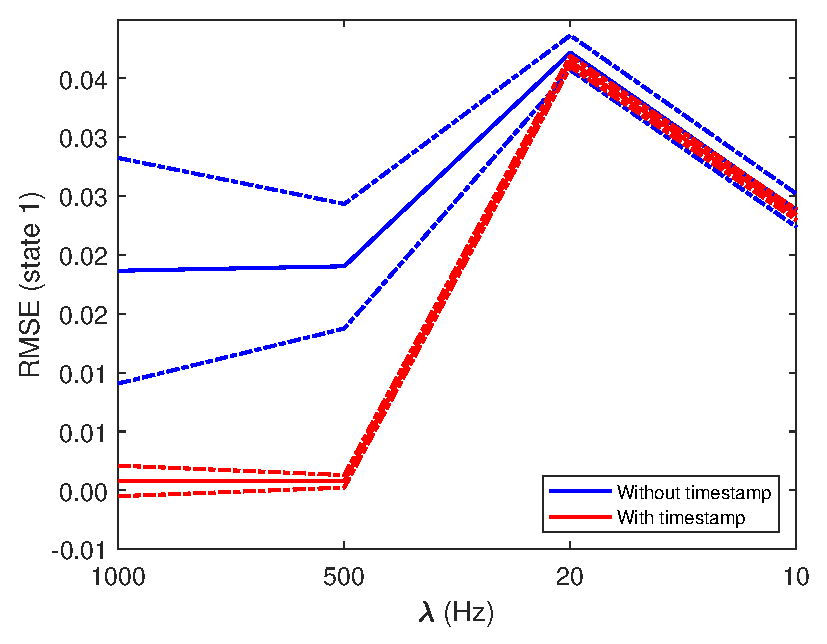
\includegraphics[width=0.49\textwidth]{Imagens/linearSamp_x1_rmse.eps}} 
%	\subfigure[]{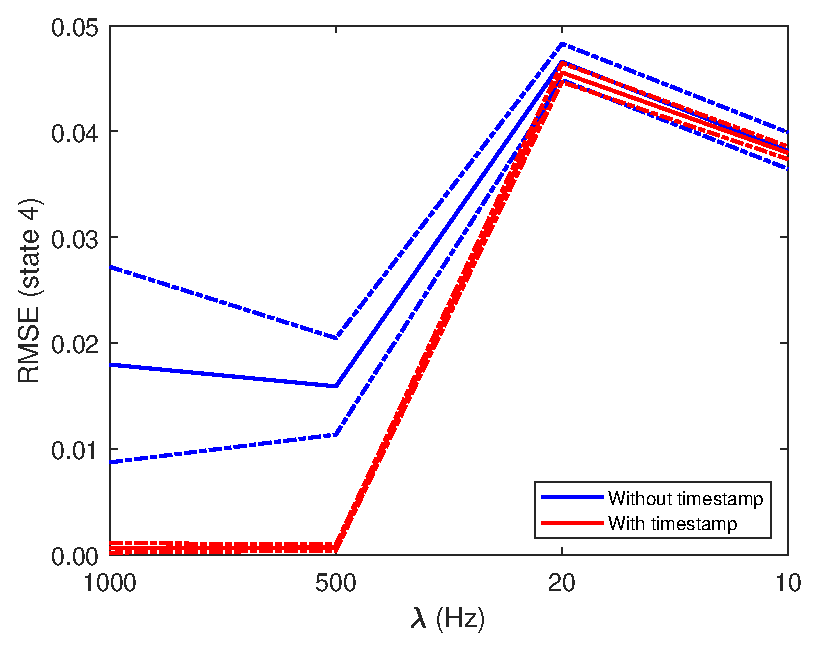
\includegraphics[width=0.49\textwidth]{Imagens/linearSamp_x4_rmse.eps}}  \\
%	\subfigure[]{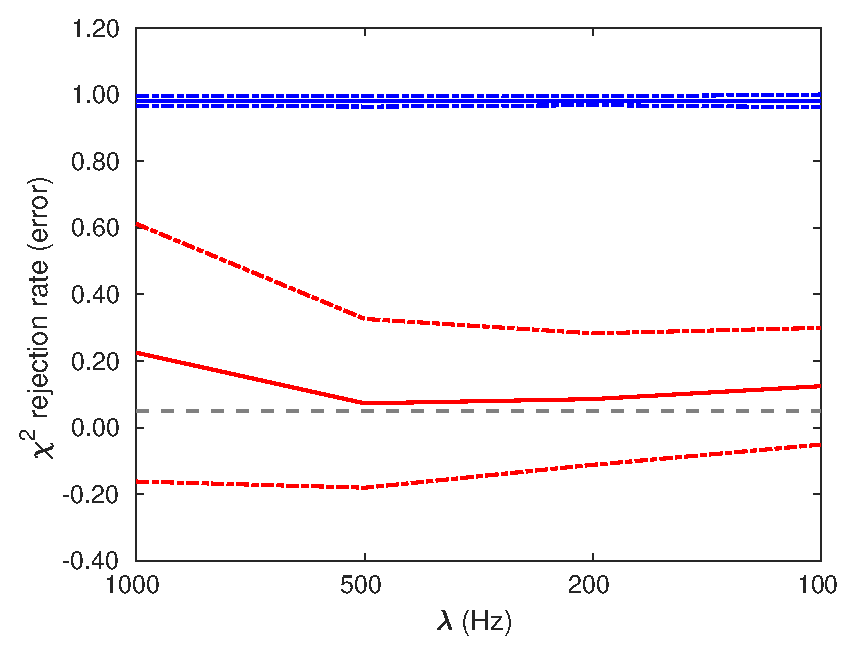
\includegraphics[width=0.49\textwidth]{Imagens/linearSamp_NEES.eps}}
%	\subfigure[]{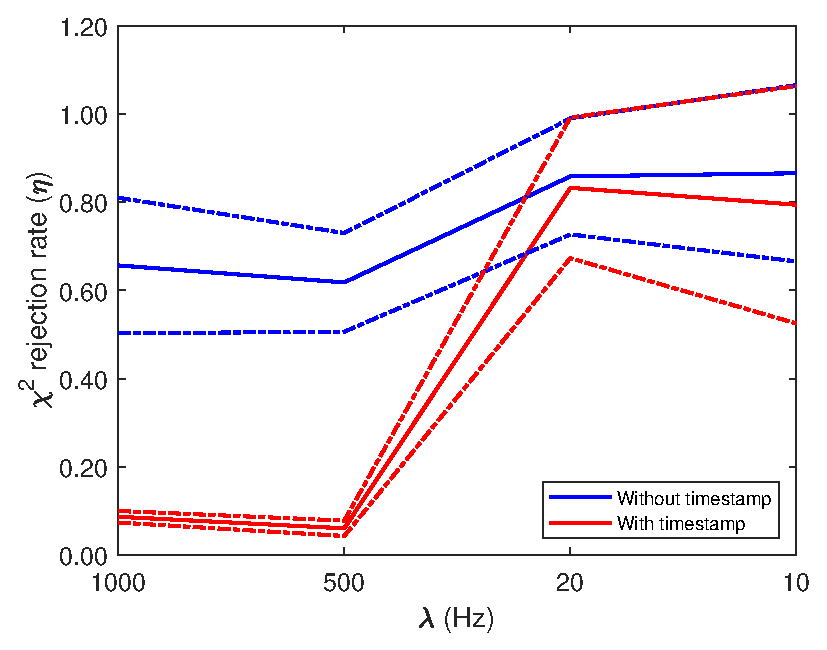
\includegraphics[width=0.49\textwidth]{Imagens/linearSamp_NIS.eps}}
%	\caption[Linear system estimation performance, as a function of input and observation SNR]{Linear system estimation performance indices with $95\%$ confidence intervals, as a function of average time interval $\lambda^{-1}$, for algorithms with (\textcolor{red}{---}) and without (\textcolor{blue}{---}) time-stamp. Accuracy values for states $x_1$ and $x_2$ are shown in (a) and (b), respectively. Consistency results are in (c) and (d) for NEES and NIS tests, respectively.}
%	\label{fig:linearSamp}
%\end{figure}

Variation of performance indices for different $\lambda$ values are shown in the second column of Figure~\ref{fig:linear_sim} and the second row of Table~\ref{tab:results_linear}. We observe the smaller differences of the means for higher $\lambda$ values, suggesting that the accuracy degradation levels caused by neglecting timestamps are higher for smaller average frequencies of the aperiodic sampled observations. That is expected, since the approximation errors of $\tilde{y}_i \approx y(t_k)$ are higher for more sparse average time intervals $1/\lambda$ and so is the additional measurement error introduced by data assimilation performed at incorrect time instants. The only exception is for state $x_1$ RMSE results for $lambda=100$ Hz. However, the sample distribution shown in Figure~\ref{fig:linear_sim} (b) has such a high variability with distant outliers, that it would be hard to draw any conclusion from this scenario. The trend shown in (e), on the other hand, is very clear. However, when it comes to effect size, we do not observe a clear trend in degradation increase. Cohen's \textit{d} values for state $x_4$ shows little difference in effect size, which is due to the variation of the standard deviations in the data from the algorithm without timestamp.

Consistency performance results in graphs (h) and (k) show that, for the simulated parameter combinations, not considering timestamp produces inconsistent estimates in all cases, while the algorithm with timestamp achieves rejection rates on NEES and NIS tests consistently closer to $5\%$. However, we observe an increase in the rejection rates for higher frequencies in the algorithm considering timestamp. It can be due to numerical errors in discretization steps performed with very small time intervals. But it would require further investigation, though.

Once again, accuracy data distributions for the algorithm not considering suggest a much higher variability, impacting negatively in estimation reliability.

\subsection{Regular and Average Irregular Time Interval Relation Variation}\label{sec:alpha-AC}

%The last linear system case study results, that is variation of $\alpha$, are shown in the third column of Figure~\ref{fig:linear_sim}. Used parameters are shown in Table~\ref{tab:params_linear_alpha} and results are presented in column (c) of Figure~\ref{fig:linear_sim}.


%\begin{table}[!ht]
%	\centering
%	\setlength{\tabcolsep}{12pt}
%	\caption[Linear system simulation parameters for $\alpha$ variation]{Linear system simulation parameters for $\alpha$ variation}
%	\begin{tabular}{c | c | c }
%		\toprule
%		SNR (dB)	& $\lambda$ (Hz) & $\alpha$ \\
%		\midrule
%		$30$		&  $500$ & $[5,\ 3,\ 2,\ 1]$  \\
%		\bottomrule
%	\end{tabular}
%	\label{tab:params_linear_alpha}
%\end{table}
%

% \begin{figure}[!htb]
%	\centering
%	\subfigure[]{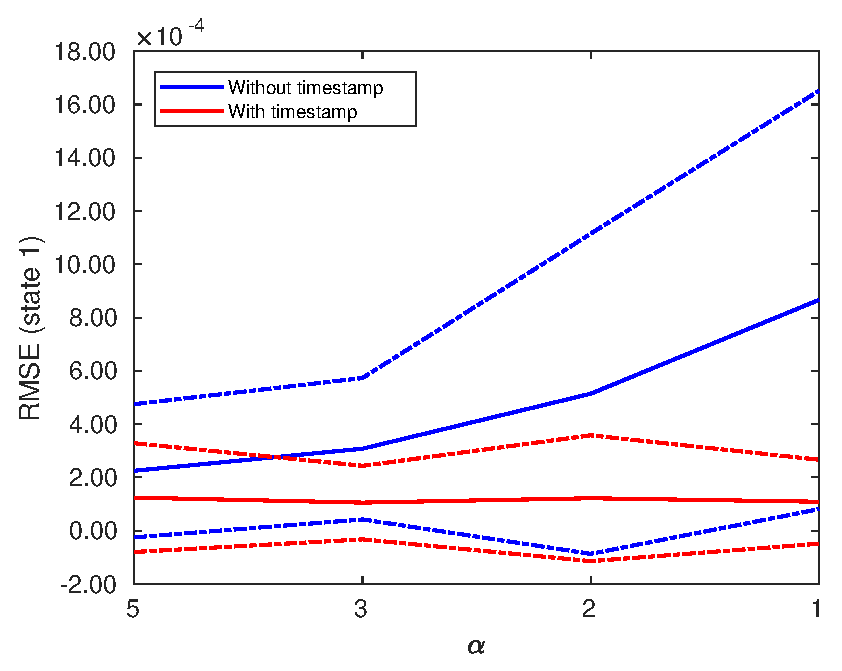
\includegraphics[width=0.49\textwidth]{Imagens/linearAlpha_x1_rmse.eps}} 
%	\subfigure[]{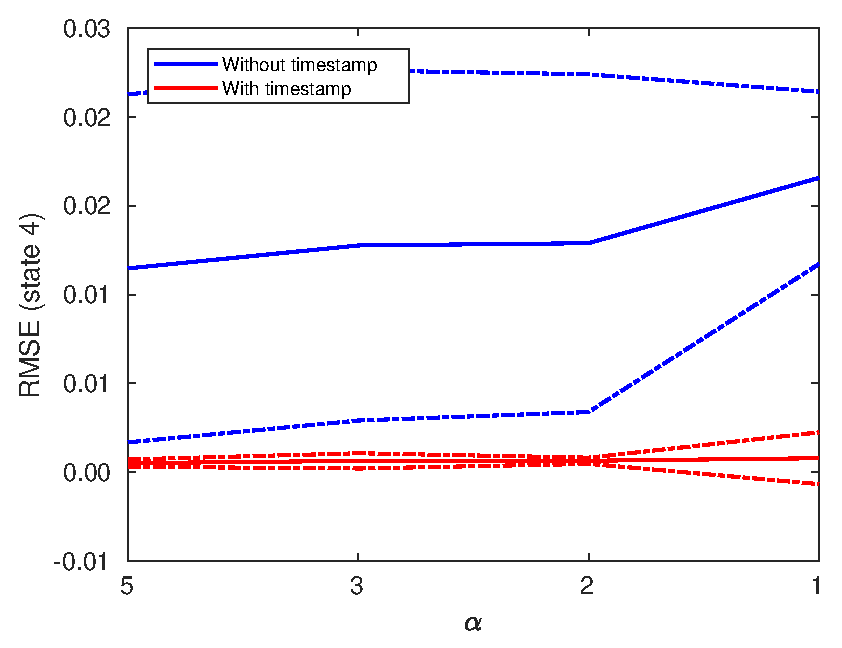
\includegraphics[width=0.49\textwidth]{Imagens/linearAlpha_x4_rmse.eps}}  \\
%	\subfigure[]{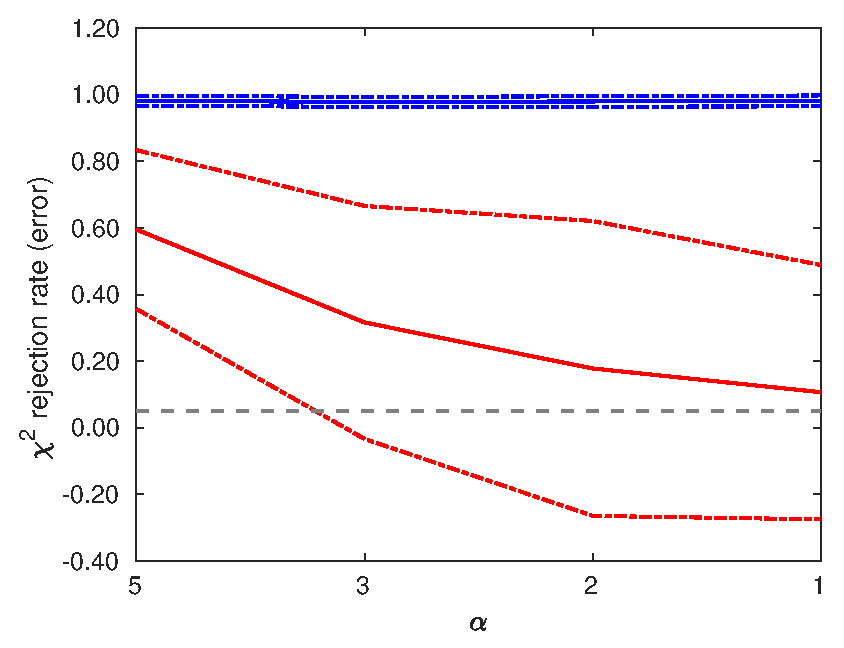
\includegraphics[width=0.49\textwidth]{Imagens/linearAlpha_NEES.eps}}
%	\subfigure[]{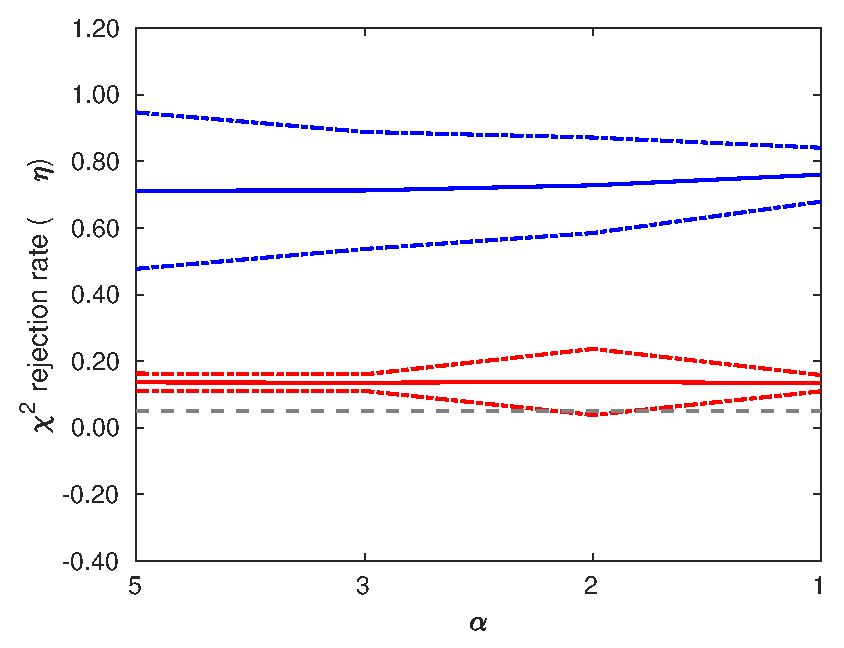
\includegraphics[width=0.49\textwidth]{Imagens/linearAlpha_NIS.eps}}
%	\caption[Linear system estimation performance, as a function of input and observation SNR]{Linear system estimation performance indices with $95\%$ confidence intervals, as a function of $\alpha$, for algorithms with (\textcolor{red}{---}) and without (\textcolor{blue}{---}) time-stamp. Accuracy values for states $x_1$ and $x_2$ are shown in (a) and (b), respectively. Consistency results are in (c) and (d) for NEES and NIS tests, respectively.}
%	\label{fig:linearAlpha}
%\end{figure}


Results obtained from increasing $\alpha$ values suggest monotonic decreasing trends for the mean of the differences in RMSE for both states $x_1$ and $x_2$, as shown in the third line of Table~\ref{tab:results_linear} and in Figure~\ref{fig:linear_sim} (c) and (f). It suggests that, the more sparse are the observation time intervals in comparison to the regular estimation time interval, that is the higher the $\alpha$, the less important it is to assimilate data at the correct time instants $t_k$. In fact, the effect size of state $x_1$ for $\alpha=5$ shows a very small practical significance in the mean difference from both algorithms. Similarly to the scenario where we vary $\lambda$ values, it can be explained by the reduction in approximation errors of $\tilde{y}_i \approx y(t_k)$ and to the fact that we considered the same SNR level for both input and output in the simulation.

By comparing the accuracy values of states $x_1$ and $x_4$, shown in Table~\ref{tab:results_linear}, we can infer a more relevant decrease in accuracy degradation for the state of the high-pass system. Whereas its mean difference decreased almost 7 times by increasing $\alpha$ from 1 to 5, that is the mean of the differences went from $6.85\times 10^{-4}$ to $0.98\times 10^{-4}$, the mean values of state $x_4$ decreased approximately 3.5 times, from $16\times 10^{-3}$ to $4.35\times 10^{-3}$. Same behavior is observed in effect size values, with a reduction of almost 4 times for state $x_1$ compared to a decrease in approximately 2 times for $x_4$.

Again, consistency test results show underestimated errors for the algorithm without timestamp systematically, whereas considering timestamp produces much more consistent estimates. An exception occurred for NEES test results, when $\alpha$ is as high as 5. We can infer that it is due to a more frequent estimation using only the forecast step, since observation time intervals are more sparse in comparison to the regular estimation time interval.

\begin{table}[!ht]
	\centering
	\footnotesize
	\setlength{\tabcolsep}{12pt}
	\caption[Linear system paired t-test results and effect size estimates for RMSE of states $x_1$ and $x_4$]{Linear system paired t-test results and effect size estimates for RMSE of states $x_1$ and $x_4$. $95\%$ confidence intervals for the mean of the differences $\mu_{\textrm{D}}$ and for Cohen's \textit{d} are shown. p-values for t-test results were all lower than $10^{-9}$, except for state $x_1$ considering $\alpha = 5$, for which it was $3.6\times 10^{-4}$.}
	\renewcommand{\arraystretch}{1.5}
	\label{tab:results_linear}
	\begin{tabular}{c | c | c c | c c }
		\toprule
		\multicolumn{2}{c}{Scenarios}	& \multicolumn{2}{c}{State 1 (RMSE difference)} 	& \multicolumn{2}{c}{State 4 (RMSE difference)} \\
		\multicolumn{2}{c}{} 		    
				& $\mu_{\textrm{D}}$  				&  Cohen's \textit{d}  	& $\mu_{\textrm{D}}$      			& Cohen's \textit{d} \\
		\midrule
		\multirow{5}{*}{SNR (dB)} 	
		& 10  	& $[2.7,\ \ 5.0]\times 10^{-4}$ 	& $[0.39,\ \ 0.97]$ 	& $[2.3,\ \ 3.8]\times 10^{-3}$ 	& $[0.52,\ \ 1.1]$ \\
		& 20  	& $[5.0,\ \ 6.9]\times 10^{-4}$ 	& $[0.97,\ \ 1.6]$ 		& $[11,\ \ 14]\times 10^{-3}$ 		& $[1.6,\ \ 2.3]$ \\
		& 40 	& $[7.4,\ \ 9.1]\times 10^{-4}$ 	& $[1.6,\ \ 2.3]$ 		& $[18,\ \ 21]\times 10^{-3}$ 		& $[2.3,\ \ 3.1]$ \\
		& 50  	& $[8.8,\ \ 10]\times 10^{-4}$  	& $[1.9,\ \ 2.6]$ 		& $[18,\ \ 21]\times 10^{-3}$ 		& $[2.8,\ \ 3.7]$ \\
		& 60  	& $[8.3,\ \ 10]\times 10^{-4}$  	& $[1.6,\ \ 2.3]$ 		& $[18,\ \ 21]\times 10^{-3}$ 		& $[2.6,\ \ 3.4]$ \\
		 						
		\midrule
		\multirow{4}{*}{$\lambda$ (kHz)} 	
		& 0.1  	& $[4.6,\ \ 7.3]\times 10^{-4}$ 	& $[0.58,\ \ 1.2]$ 		& $[3.7,\ \ 4.4]\times 10^{-2}$ 	& $[2.0,\ \ 2.7]$ \\
		& 0.3  	& $[6.5,\ \ 8.2]\times 10^{-4}$ 	& $[1.4,\ \ 2.0]$ 		& $[3.1,\ \ 3.7]\times 10^{-2}$ 	& $[2.1,\ \ 2.9]$ \\
		& 0.5 	& $[6.1,\ \ 8.1]\times 10^{-4}$ 	& $[1.1,\ \ 1.7]$ 		& $[1.6,\ \ 1.9]\times 10^{-2}$ 	& $[2.3,\ \ 3.1]$ \\
		& 1  	& $[2.1,\ \ 3.5]\times 10^{-4}$  	& $[0.46,\ \ 1.0]$ 		& $[0.66,\ \ 0.78]\times 10^{-2}$ 	& $[2.0,\ \ 2.7]$ \\

		\midrule
		\multirow{4}{*}{$\alpha$} 	
		& 1  	& $[5.9,\ \ 7.8]\times 10^{-4}$ 	& $[1.1,\ \ 1.8]$ 		& $[15,\ \ 17]\times 10^{-3}$ 		& $[2.5,\ \ 3.2]$ \\
		& 2  	& $[3.1,\ \ 4.2]\times 10^{-4}$ 	& $[0.96,\ \ 1.6]$ 		& $[8.9,\ \ 11]\times 10^{-3}$ 		& $[1.9,\ \ 2.6]$ \\
		& 3 	& $[1.6,\ \ 2.5]\times 10^{-4}$ 	& $[0.56,\ \ 1.1]$ 		& $[5.6,\ \ 6.7]\times 10^{-3}$ 	& $[1.7,\ \ 2.4]$ \\
		& 5  	& $[0.46,\ \ 1.5]\times 10^{-4}$  	& $[0.088,\ \ 0.65]$ 	& $[3.8,\ \ 4.9)\times 10^{-3}$ 	& $[1.3,\ \ 2.0]$ \\

													     
		\bottomrule
	\end{tabular}

\end{table}

\clearpage
\begin{figure}[H]
	\centering
	\subfigure[SNR variation]{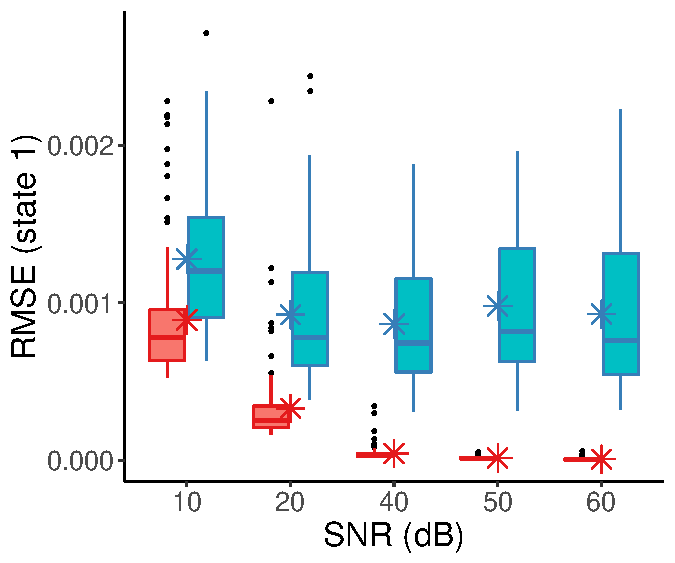
\includegraphics[width=0.32\textwidth]{Imagens/Rlinear_noise_x1.pdf}} 
	\subfigure[$\lambda$ variation]{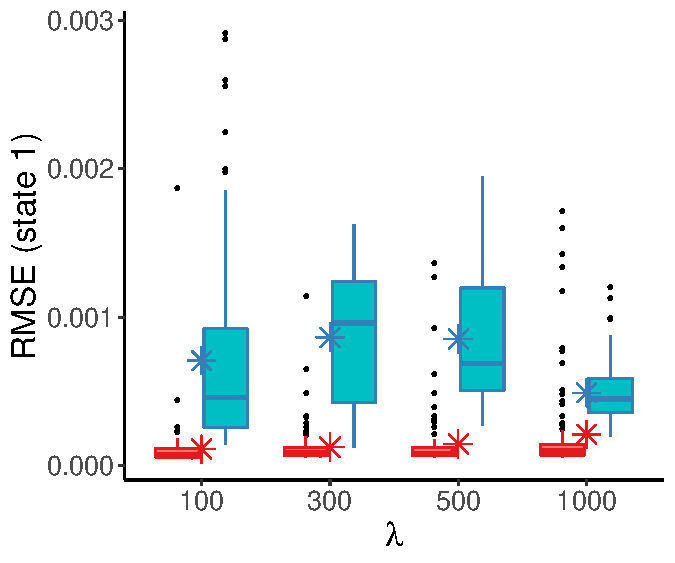
\includegraphics[width=0.32\textwidth]{Imagens/Rlinear_lambda_x1.pdf}}  
	\subfigure[$\alpha$ variation]{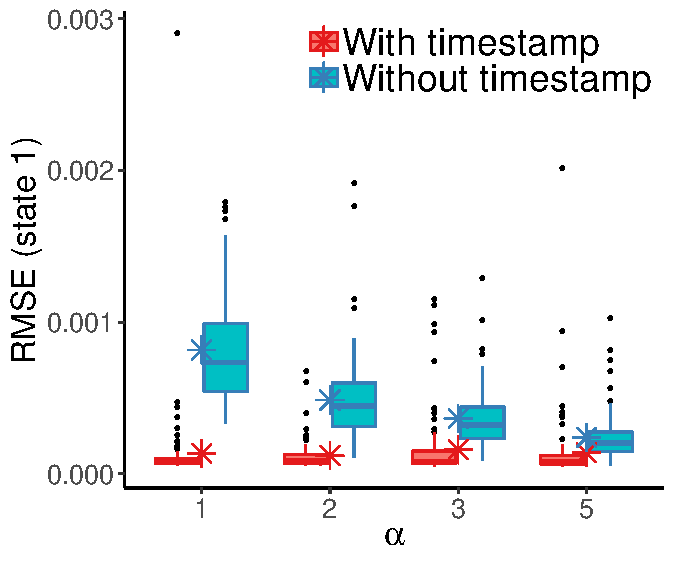
\includegraphics[width=0.32\textwidth]{Imagens/Rlinear_alpha_x1.pdf}} \\
	\subfigure[SNR variation]{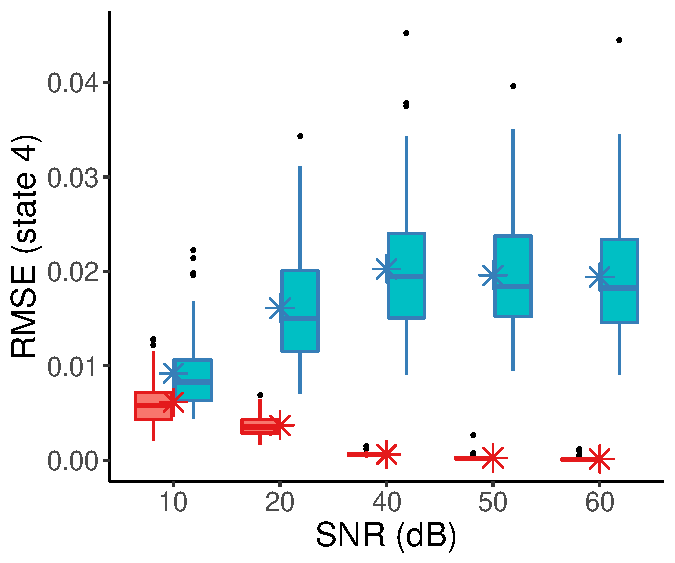
\includegraphics[width=0.32\textwidth]{Imagens/Rlinear_noise_x4.pdf}} 
	\subfigure[$\lambda$ variation]{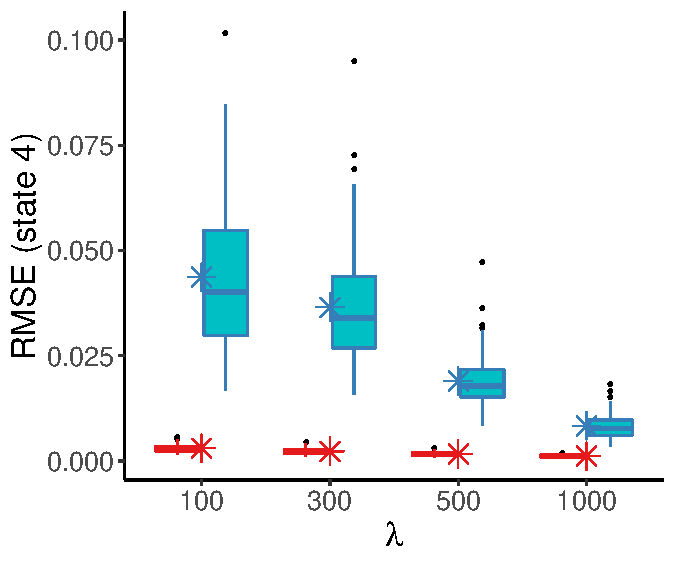
\includegraphics[width=0.32\textwidth]{Imagens/Rlinear_lambda_x4.pdf}}  
	\subfigure[$\alpha$ variation]{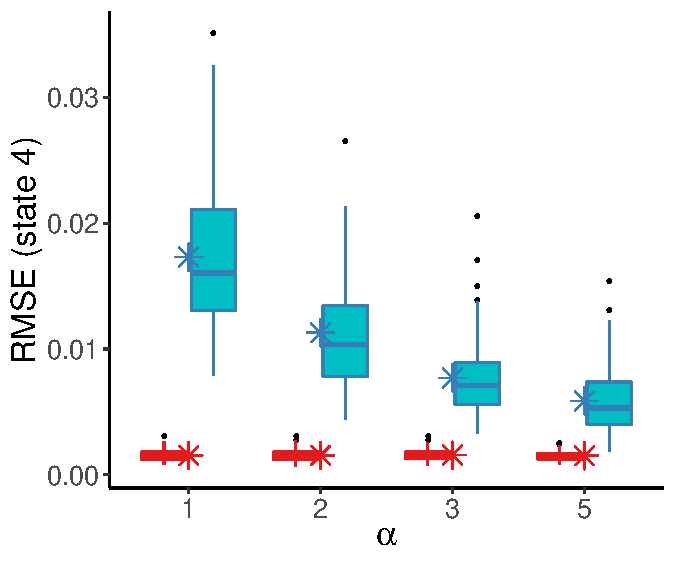
\includegraphics[width=0.32\textwidth]{Imagens/Rlinear_alpha_x4.pdf}} \\
	\subfigure[SNR variation]{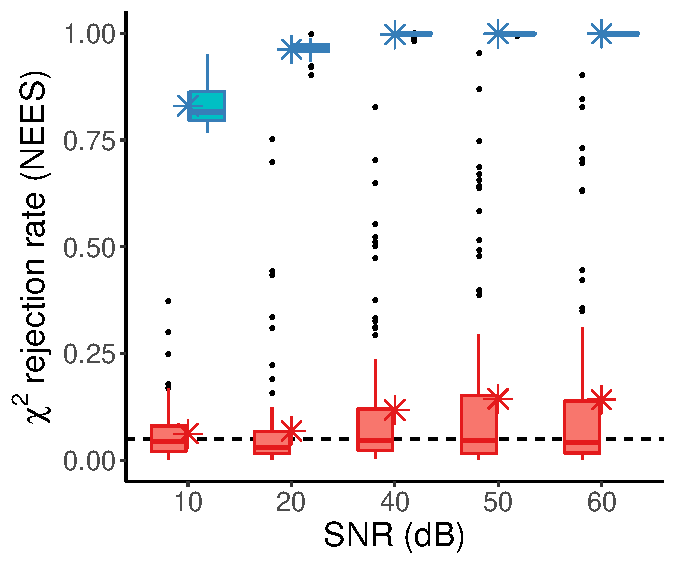
\includegraphics[width=0.32\textwidth]{Imagens/Rlinear_noise_chix.pdf}} 
	\subfigure[$\lambda$ variation]{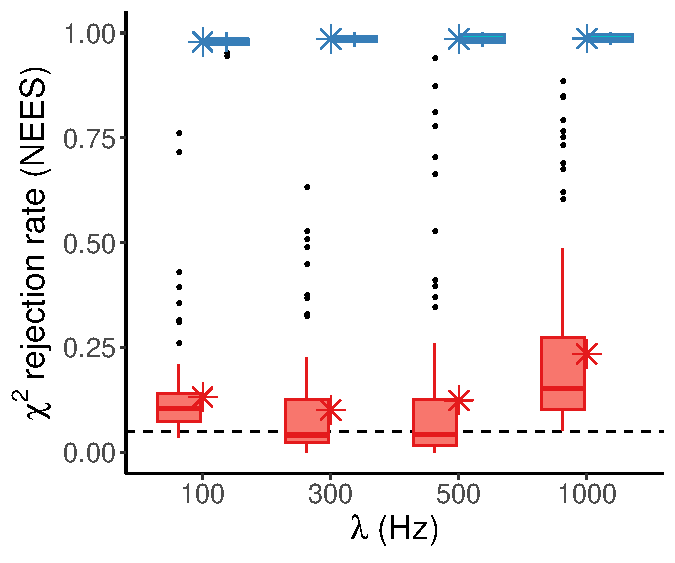
\includegraphics[width=0.32\textwidth]{Imagens/Rlinear_lambda_chix.pdf}}  
	\subfigure[$\alpha$ variation]{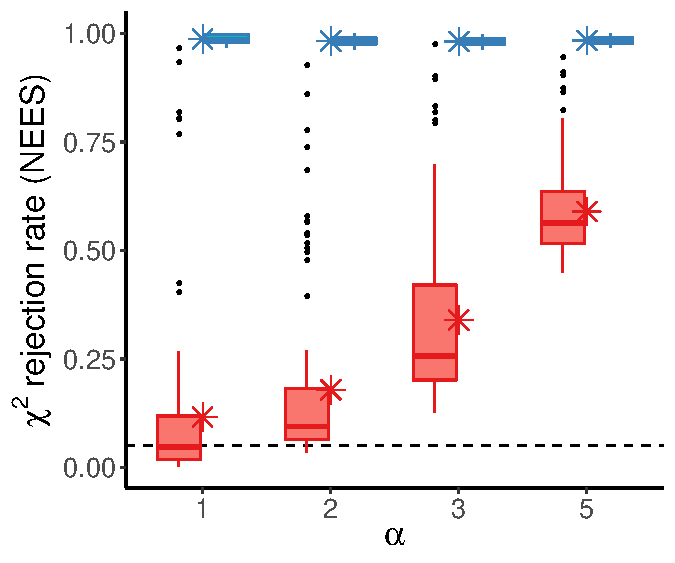
\includegraphics[width=0.32\textwidth]{Imagens/Rlinear_alpha_chix.pdf}} \\
	\subfigure[SNR variation]{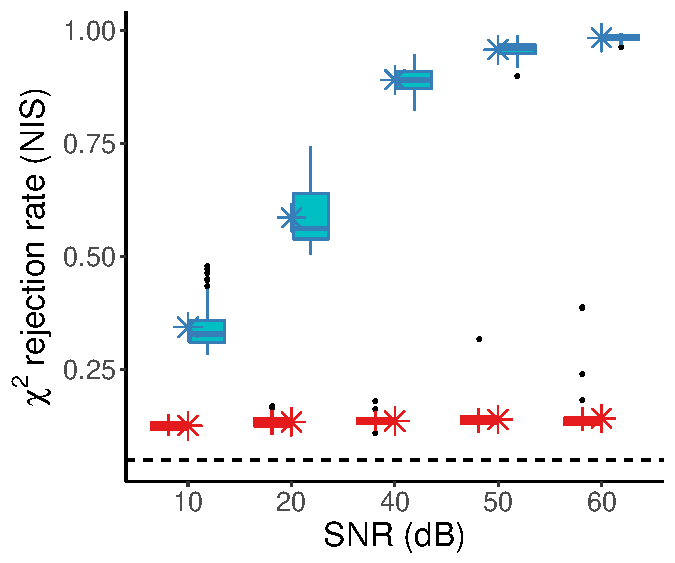
\includegraphics[width=0.32\textwidth]{Imagens/Rlinear_noise_chiy.pdf}} 
	\subfigure[$\lambda$ variation]{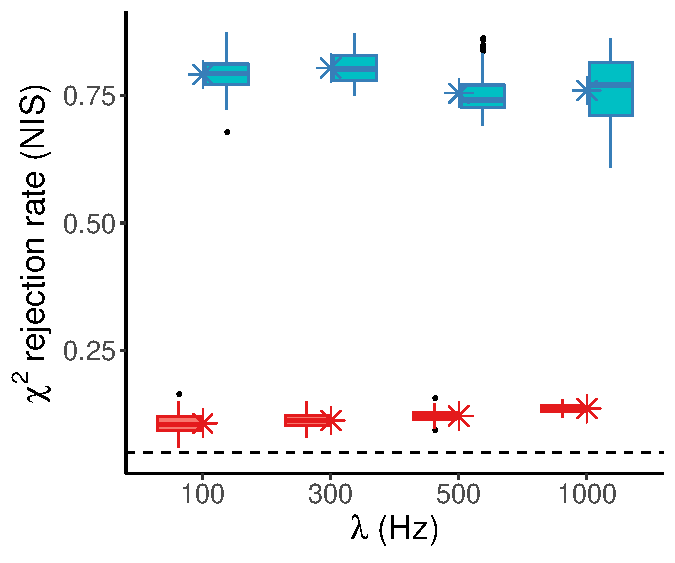
\includegraphics[width=0.32\textwidth]{Imagens/Rlinear_lambda_chiy.pdf}}  
	\subfigure[$\alpha$ variation]{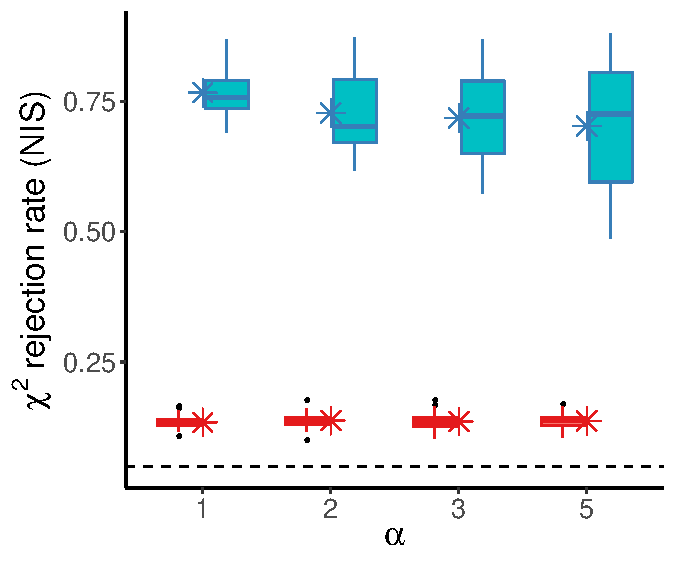
\includegraphics[width=0.32\textwidth]{Imagens/Rlinear_alpha_chiy.pdf}} \\
	\caption[Linear system estimation performance comparison]{Box and whiskers plots for the linear system estimation results, as a function of SNR (a,d,g,j), $\lambda$ (b,e,h,k) and $\alpha$ (c,f,i,l), considering (red) and not considering (blue) timestamps. Mean values are presented in asterisks. Horizontal gray dashed lines for consistency results represents the $5\%$ significance level limits.}
	\label{fig:linear_sim}
\end{figure}



%\begin{figure}[H]
%	\centering
%	\subfigure[SNR variation]{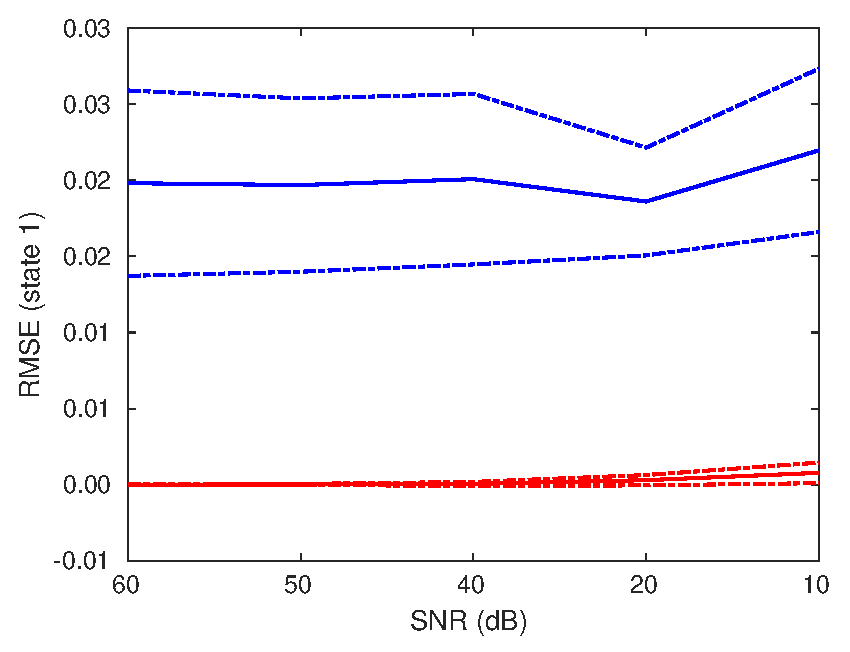
\includegraphics[width=0.32\textwidth]{Imagens/linearNoise_x1_rmse.eps}} 
%	\subfigure[$\lambda$ variation]{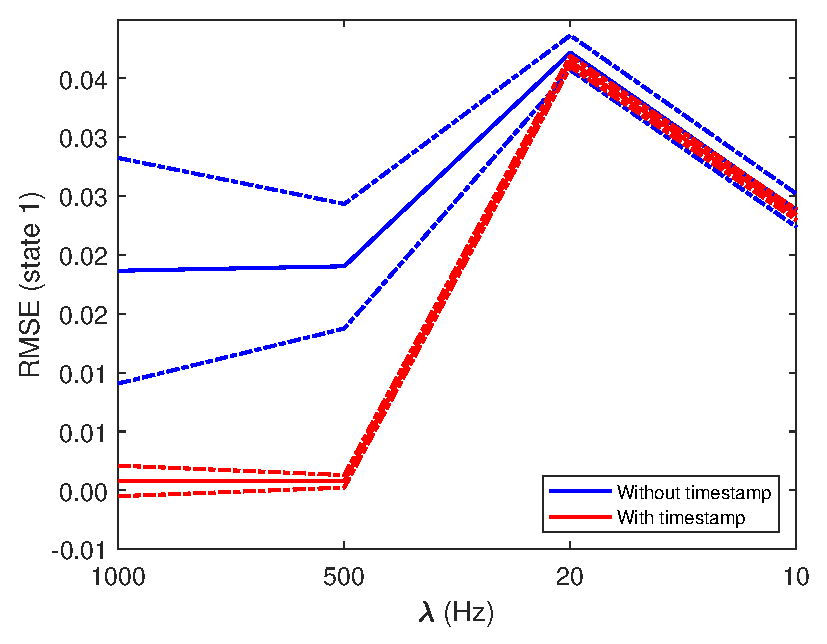
\includegraphics[width=0.32\textwidth]{Imagens/linearSamp_x1_rmse.eps}}  
%	\subfigure[$\alpha$ variation]{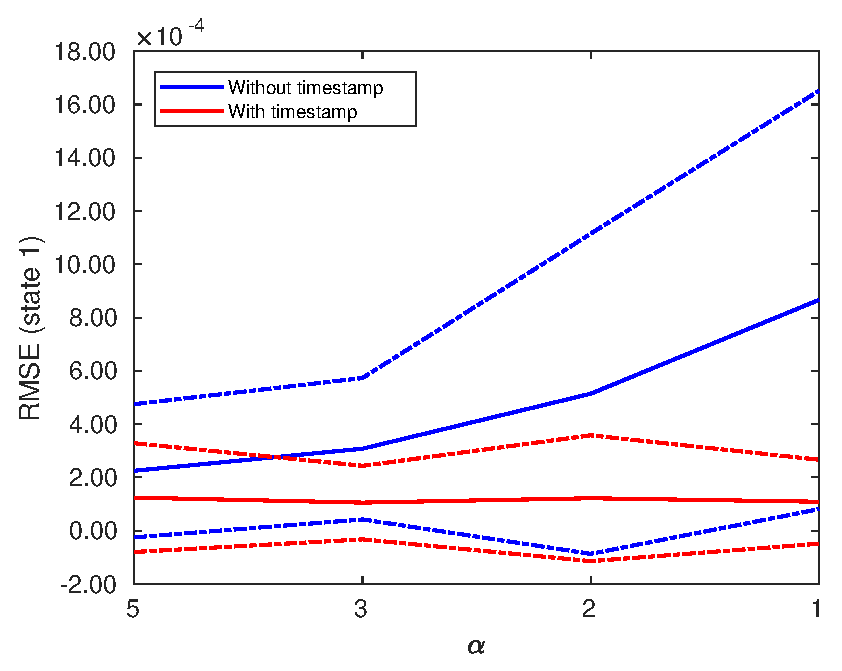
\includegraphics[width=0.32\textwidth]{Imagens/linearAlpha_x1_rmse.eps}} \\
%	\subfigure[SNR variation]{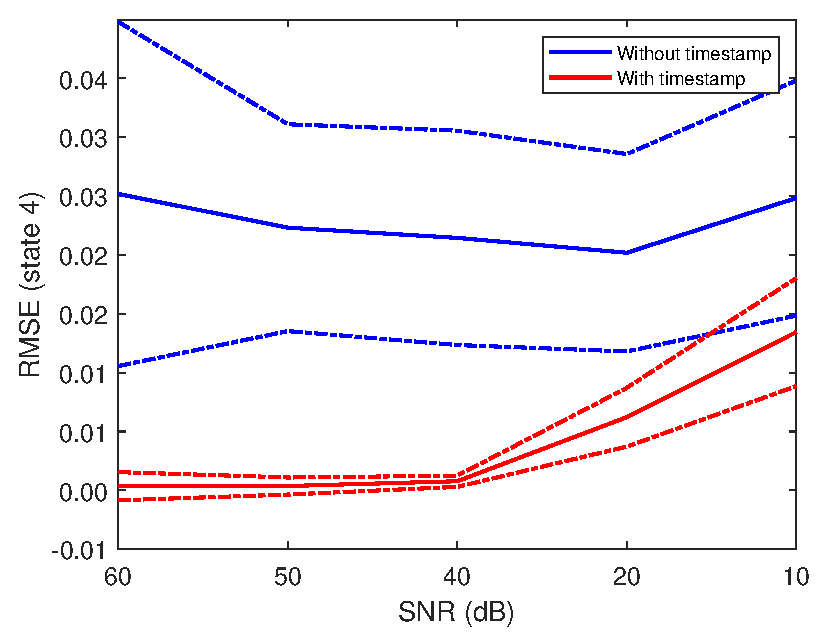
\includegraphics[width=0.32\textwidth]{Imagens/linearNoise_x4_rmse.eps}} 
%	\subfigure[$\lambda$ variation]{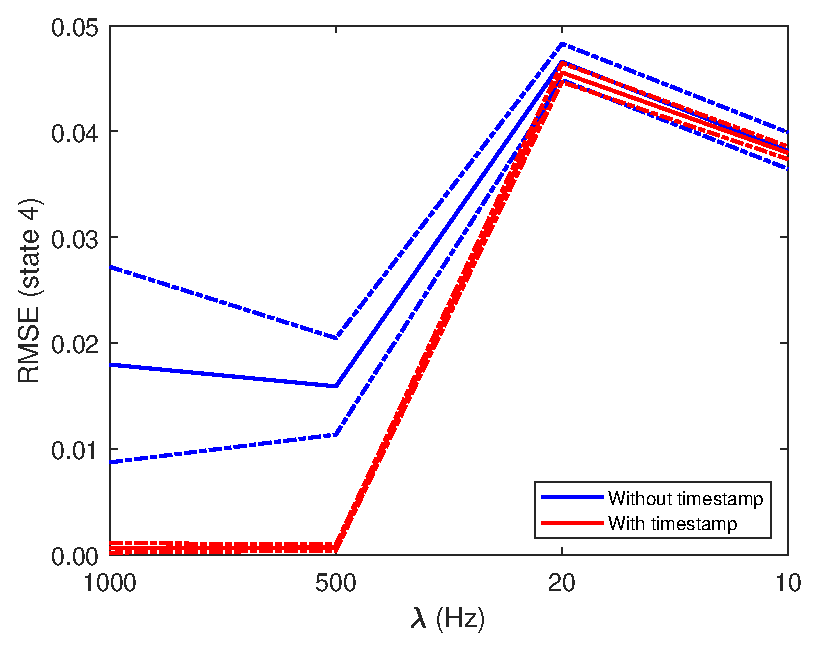
\includegraphics[width=0.32\textwidth]{Imagens/linearSamp_x4_rmse.eps}}  
%	\subfigure[$\alpha$ variation]{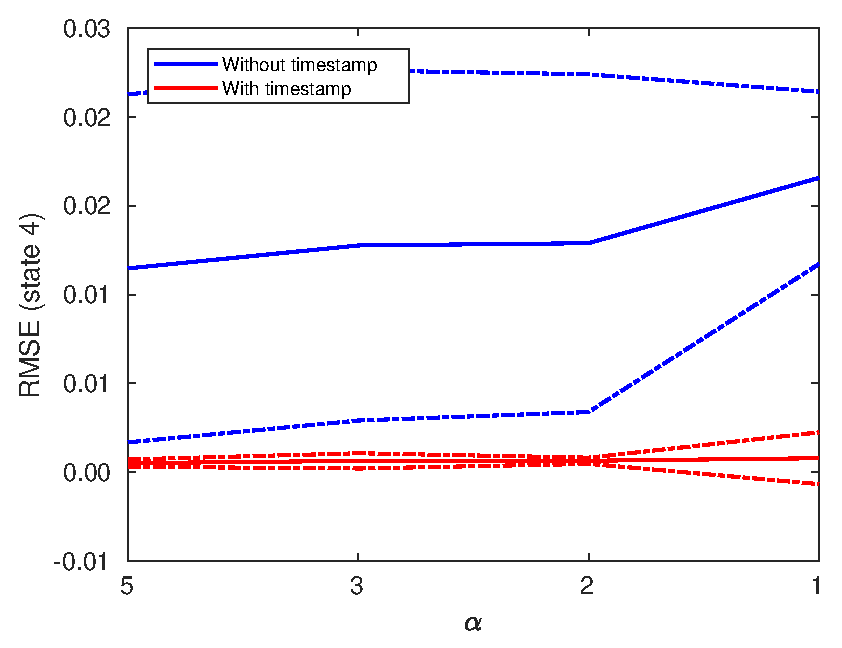
\includegraphics[width=0.32\textwidth]{Imagens/linearAlpha_x4_rmse.eps}} \\
%	\subfigure[SNR variation]{\includegraphics[width=0.32\textwidth]{Imagens/linearNoise_NEES.eps}} 
%	\subfigure[$\lambda$ variation]{\includegraphics[width=0.32\textwidth]{Imagens/linearSamp_NEES.eps}}  
%	\subfigure[$\alpha$ variation]{\includegraphics[width=0.32\textwidth]{Imagens/linearAlpha_NEES.eps}} \\
%	\subfigure[SNR variation]{\includegraphics[width=0.32\textwidth]{Imagens/linearNoise_NIS.eps}} 
%	\subfigure[$\lambda$ variation]{\includegraphics[width=0.32\textwidth]{Imagens/linearSamp_NIS.eps}}  
%	\subfigure[$\alpha$ variation]{\includegraphics[width=0.32\textwidth]{Imagens/linearAlpha_NIS.eps}} \\
%	\caption[Linear system estimation performance comparison]{Linear system estimation mean performance indices with $95\%$ confidence intervals, as a function of SNR (a,d,g,j), $\lambda$ (b,e,h,k) and $\alpha$ (c,f,i,l), considering (\textcolor{red}{---}) and not considering (\textcolor{blue}{---}) time-stamp. RMSE results are shown in the first ($x_1$) and second ($x_4$) rows. Consistency results are in third (NEES)) and fourth (NIS) rows. Horizontal gray dashed lines represent the $5\%$ significance level for the consistency tests.}
%	\label{fig:linear_sim_old}
%\end{figure}


%
%\subsection{Average Time Delay}\label{sec:dt-AC}
%
%\todo[inline,caption={Falta variar o atraso nas medi��es}]{Ainda ter� uma se��o com a varia��o do time-delay e seu impacto no desempenho}


\section{Nonlinear System: Unicycle Position}

We now consider a nonlinear system given by a nonholomonic moving unicycle robot, whose position in the $xy$-plane must be estimated. In many real target tracking problems such as this, measurements are available by unsynchronized cameras through an internet network, for instance. In other applications multiple GPS sensors might be used in a centralized architecture without data alignment or association. These configurations are susceptible to sampling irregularities, which motivates our choice. On the other hand, inertial sensors responsible for input data, such as girometers and accelerometers transmit data regularly, but usually with lower SNR values.

\subsection{System Description}

Consider a nonholomonic moving robot, with the cinematic process model given by

\setlength{\abovedisplayskip}{0.5pt}

\begin{equation}\label{eq:sistema}
\begin{split}
\dot{p}_\textrm{x} & = v\cos (\theta),\\
\dot{p}_\textrm{y} & = v\sin (\theta),\\
\dot{\theta}  & = u_1(t),\\
\dot{v} & = u_2(t),
\end{split}
\end{equation}

\noindent
where $p_\textrm{x}$ and $p_\textrm{y}$ are the position coordinates, $\theta$ the angular orientation, $v$ the linear velocity and inputs $u_1$ and $u_2$ are the angular velocity $\omega$ and the linear acceleration $a$, respectively. Figure~\ref{fig:robot} shows a schematic of the robot and its states,

\begin{figure}[!htb]
	\centering
	\includegraphics[width=0.4\textwidth]{Imagens/Nonholomonic-robot.pdf}
	\caption[Nonholomonic robot system representation]{Nonholomonic robot system representation. The system states $p_\textrm{x}$, $p_\textrm{y}$, $v$ and $\theta$ are highlighted.}
	\label{fig:robot}
\end{figure} 

The system described by (\ref{eq:sistema}) is discretized by a fourth order Runge-Kutta method as described in Section~\ref{sec:discretization} and the discrete-time state vector $x_i$ is given by $x_i \overset{\Delta}{=} [p_{\textrm{x},i}\ \  p_{\textrm{y},i}\ \  \theta_i\ \  v_i]^T$, where subscript $i$ indicate discrete instants $iT$.

The observation model $y(t_k) \in \mathbb{R}^2$ 

\begin{equation}
y(t_k) = 
\begin{bmatrix}
p_\textrm{x}(t_k) \\
p_\textrm{y}(t_k)
\end{bmatrix}+v(t_k), \\
\end{equation}

\noindent
is given by the position coordinates, and $\rho(v(t_k)) = \mathcal{N} (0,R_{t_k})$ is the observation noise PDF, with zero mean and covariance $R_{t_k}$. Discrete time instants $t_k$ are determined by random time intervals $h_k$, that is $t_{k+1}=t_k+h_k$. When time-stamp information about $t_k$ is not available, the observation vector is approximated by $\tilde{y}_i \approx y(t_k)$, where $i$ is the index of the next time instant, multiple of $T$.

Input vector $u_i = [\omega_i\ \ a_i]^T$ is measured by a girometer and accelerometer, respectively. We assume that 

\begin{equation}\label{eq:entrada}
u_i = \tilde{u}_i - w_i,
\end{equation}

\noindent
where $\tilde{u}$ represent the sensors' measured values and $\rho(w_i) = \mathcal{N} (0, Q_i)$ is the corresponding noise PDF, with zero mean and covariance $Q_i$. 

We simulate 60 seconds of robot movement, considering a step size of $\delta t_{\textrm{sim}} = 10^{-4}$, generating $600.000$ samples to mimic the continuous system dynamics. Input signals are generated arbitrarily according to Figure~\ref{fig:entrada}. 

\begin{figure}[!htb]
	\centering
	\subfigure[]{\includegraphics[width=0.75\textwidth]{Imagens/entradas1.eps}} \\
	\subfigure[]{\includegraphics[width=0.75\textwidth]{Imagens/entradas2.eps}}  
	\caption[Simulation input signals]{Simulation input signals. (a) shows temporal sequence of angular velocity $\omega$ and (b) shows linear acceleration $a$.}
	\label{fig:entrada}
\end{figure}

Accuracy metrics for the unicycle position system is a modification of the RMSE defined in (\ref{eq:rmse}), to reflect error in $xy$-plane position, given by:

\begin{equation}\label{eq:pos_rmse}
RMSE_{\textrm{position}} = \frac{ \sum_{i=1}^N \sqrt{(\hat{p}_{\textrm{x},i}-p_{\textrm{x},i})^2+(\hat{p}_{\textrm{y},i}-p_{\textrm{y},i})^2}}{N},
\end{equation}

\noindent
where $\hat{p}_{\textrm{x},i}$ and $\hat{p}_{\textrm{y},i}$ are position estimates at regularly spaced time intervals $T$, $p_{\textrm{x},i}$ and $p_{\textrm{y},i}$ are true position coordinates of the unicycle, at the same time instants and $N$ is the total amount of estimates.


%sampling time intervals $h_k$ are simulated by the exponential probability distribution function from Matlab\texttrademark \ and approximated to the nearest discrete time instant, from the 600,000 available samples. 


\subsection{Single Realization Analysis}

Figure~\ref{fig:exukf} (a) shows the robot trajectory on the $xy$-plane for the given input signals, leaving from point $(0,0)$, as well as a realization of noisy and aperiodic measurements as red dots, with signal-to-noise ratio of $\textrm{SNR\textsubscript{y}} = 30$ dB and $\lambda=3.33$ Hz. The dashed blue line represents UKF estimation, considering timestamp, $\alpha=5$ and $\textrm{SNR\textsubscript{u}} = 10 \textrm{ dB}$. 

Figure~\ref{fig:exukf} (b) shows a timespan from $0$ to $1.5$ seconds of a position RMSE realization, considering $\lambda=0.5$, $\alpha=2$, $\textrm{SNR\textsubscript{y}} = 40 \textrm{ dB}$ and $\textrm{SNR\textsubscript{u}} = 20 \textrm{ dB}$, for the UKF considering and not considering timestamp. Black dots represent the regular time instants $kT$ whereas the asterisks on $x$-axis and dashed vertical lines match the exact measurement instants $t_k$. The first two measurements, before 0.25 seconds, are very close to the first regular time instant $1T = 0.25 \textrm{ s}$ and thus cause no significant difference on performance. It is expected, since the approximation error due to $\tilde{y}_i \approx y(t_k)$ is irrelevant. The third measurement, taking place around $0.8$ seconds, when assimilated correctly reduces the estimate error at the correct instant. When assimilated at the next estimation time instant, the position error is not decreased appropriately. At the instant of the fourth measurement, around $1.1$ seconds, we can see another effect of assimilating the measurement at the correct time, with the red line decreasing slightly. 



\begin{figure}[!htb]
	\centering
	\subfigure[]{\includegraphics[width=0.49\textwidth]{Imagens/exemplo_03_30db_desloc.eps}} 
	\subfigure[]{\includegraphics[width=0.49\textwidth]{Imagens/RobotJEvolution2.eps}}  
	\caption[Single realization of unicycle position estimation]{(a) True position (\textcolor{black}{---}), noisy measurements (\textcolor{red}{$\cdot$}) and UKF estimates (\textcolor{blue}{- -}) considering timestamp, for a measurement noise of SNR\textsubscript{y} $= 30$ dB, $\lambda=0.3$ s and $\alpha=5$. (b) Temporal cut from 0 to 1.5 seconds, for a realization of $J$ of both estimators, with and without timestamp. Asterisks on $x$ axis and vertical dashed lines match the measurement sampling instants $t_k$. Black dots represent the regular estimation instants, same as input regular sampling instants.}
	\label{fig:exukf}
\end{figure}


%\begin{figure}[!htb]
%	\centering
%	\includegraphics[width=0.7\textwidth]{Imagens/exemplo_03_30db_desloc.eps}
%	\caption[True position, noisy measurements and UKF estimates]{True position (\textcolor{black}{---}), noisy measurements (\textcolor{red}{$\cdot$}) and UKF estimates (\textcolor{blue}{- -}) considering time-stamp, for a measurement noise of SNR\textsubscript{y} $= 30$ dB, $\lambda=0.3$ s and $\alpha=5$.}
%	\label{fig:exukf}
%\end{figure} 



%\begin{figure}[!htb]
%	\centering
%	\includegraphics[width=0.7\textwidth]{Imagens/RobotJEvolution.eps}
%	\caption[Performance index temporal cut for one realization]{Temporal cut from 0 to 1.5 seconds, for a realization of $J$ of both estimators, with and without time-stamp. Asterisks on $x$ axis and vertical dashed lines match the measurement sampling instants $t_k$. Black dots represent the regular estimation instants, same as input regular sampling instants.}
%	\label{fig:realizacaoJ}
%\end{figure} 

In the next sections we perform Monte Carlo simulations, with 1000 runs per parameter combination, for the scenarios described in Section~\ref{sec:scenarios}. Simulation parameters used for the nonlinear system are shown in Table~\ref{tab:params_robot}. For all cases, input SNR is constant at $20$ dB. Paired t-test results and effect size of the mean differences for position RMSE are shown in Table~\ref{tab:results_robot}. Figure~\ref{fig:robot_sim} summarizes information of all results, with box and whiskers plots of numerical simulation data for each scenario. First row of graphs shows accuracy results for position RMSE, as defined in (\ref{eq:pos_rmse}). Second and third rows present the consistency results for NEES and NIS tests, respectively, as described in Section~\ref{sec:metrics}. Red plots are for the algorithm that considers timestamp and blue for the one without timestamp.

\begin{table}[!ht]
	\centering
	\setlength{\tabcolsep}{12pt}
	\caption[Sets of parameters for nonlinear system simulation parameters]{Sets of parameters for unicycle position estimation simulation parameters}
	\renewcommand{\arraystretch}{1.5}
	\small
	\begin{tabular}{c | c | c | c}
		\toprule
		Scenario 		& SNR observations (dB)	& $\lambda$ (Hz) & $\alpha$ \\
		\midrule
		SNR variation 	& $[100, \ 80,\ 60,\ 40,\ 20,\ 10]$ &  $10$ & $2$  \\
		$\lambda$ variation		&	$40$ & 	 $[10, \ 5,\ 0.33,\ 2.5,\ 2,\ 1.67]$ & $2$  \\
		$\alpha$ variation	&$40$ 				&  $10$ & $[10, \ 5,\ 2,\ 1]$  \\
		\bottomrule
	\end{tabular}
	\label{tab:params_robot}
\end{table}


%\begin{figure}[!htb]
%	\centering
%	\includegraphics[width=0.8\textwidth]{Imagens/J_umarealizacao-timedelay.eps}
%%%	\caption[entrada]{Recorte temporal de 1 a 1.3 segundo, do �ndice J de uma realiza��o dos dois estimadores, com e sem carimbo de tempo. Os asteriscos no eixo $x$ representam os instantes de amostragem das observa��es $t_k$. Os pontos pretos apresentados nas linhas representam os instantes de tempo regulares de amostragem da entrada}
%	\label{fig:realizacaoJ2}
%\end{figure} 



%\setlength{\abovedisplayskip}{0.5pt}
%
%\begin{equation}\label{eq:sistema}
%\begin{split}
%\dot{\delta_e} & = -\tau^{-1},\\
%\dot{W} & = Z_{de}\delta_e + Z_wW + S_0q,\\
%\dot{q}  & = S_1 \delta_e + S_2 W + S_3q,\\
%\end{split}
%\end{equation}
%\noindent

\subsection{Measurement Signal-to-Noise Ratio Variation}\label{sec:ruido-robo}

%In this subsection we compare the estimation performance impact of considering time-stamp in the algorithm, by varying the measurement noise level. The signal-to-noise ratio for the input sensors, the measurement average time interval and $\alpha$ are held constant. Table~\ref{tab:params_robot_snr} shows the parameters used in simulation.

%\begin{table}[!ht]
%	\centering
%	\setlength{\tabcolsep}{12pt}
%	\caption[Nonlinear system simulation parameters for SNR variation]{Unicycle position estimation simulation parameters for observation SNR variation}
%	\begin{tabular}{c | c | c | c }
%		\toprule
%		SNR observations (dB)	& SNR input (dB) & $\lambda$ (Hz) & $\alpha$ \\
%		\midrule
%		$[100, \ 80,\ 60,\ 40,\ 20,\ 10]$ & $20$ & $10$ & $2$  \\
%		\bottomrule
%	\end{tabular}
%	\label{tab:params_robot_snr}
%\end{table}



% \begin{figure}[!htb]
%	\centering
%	\subfigure[]{\includegraphics[width=0.49\textwidth]{Imagens/noise.eps}} 
%	\subfigure[]{\includegraphics[width=0.49\textwidth]{Imagens/noise.eps}}  \\
%	\subfigure[]{\includegraphics[width=0.49\textwidth]{Imagens/noise.eps}} 
%	\subfigure[]{\includegraphics[width=0.49\textwidth]{Imagens/noise.eps}}     
%
%	\caption[Robot tracking performance, as a function of measurement noise]{Robot tracking performance indices with $95\%$ confidence intervals, as a function of measurement noise, for both UKF algorithms considering (\textcolor{red}{---}) and not considering (\textcolor{blue}{---}) time-stamp. Accuracy values for states $P_{\textrm{x}}$ and  $P_{\textrm{y}}$ are shown in (a) and (b), respectively. Consistency results are in (c) and (d) for NEES and NIS tests, respectively.}
%	\label{fig:robot_noise}
%\end{figure}

Results from the first row of Table~\ref{tab:results_robot} and the first column of Figure~\ref{fig:robot_sim} show the variation in performance for the different measurement SNR levels simulated. Both algorithms, in most cases, have their estimate error increased, when measurement data is contaminated with higher noise levels, as expected. We observe from Table~\ref{tab:results_robot}, however, that the mean differences are higher when there is less noise, in favor of considering timestamp in the estimation process. The effect size results also suggest an upper bound for such difference. It can be explained similarly to what was observed in the linear system. The higher the SNR levels, the more relevant are the approximation errors of $\tilde{y}_i \approx y(t_k)$. When measurements are highly contaminated with noise, these approximation errors get irrelevant for the estimation process, and both algorithms perform similarly. In fact, there is smaller practical significance in the results for low SNR levels, as shown by Cohen's \textit{d} values.

Same behavior can be observed in the consistency tests results. Estimates are inconsistent for the algorithm without timestamp only for higher SNR. When noise levels increase, both algorithms have similar consistency results. Graph (g) shows a slight inconsistency in the estimation of the algorithm with timestamp, for $100$ db SNR. It might be due to numerical errors and approximations caused by very small measurement covariances, when there is virtually no noise in data.
 
From the box and whiskers plots for position RMSE, we can observe once again higher variability in the results obtained from neglecting timestamps. A more significant presence of outliers is also apparent. Both aspects indicate less reliable estimation performance.


\subsection{Average Sampling Rate Variation}\label{sec:lambda-robot}

%We now consider the variation of the average sampling rate that observations are taken, maintaining the other parameters constant, according to Table~\ref{tab:params_robot_lambda}. Results for accuracy and consistency are shown in column (b) of .
%%
%\begin{table}[!ht]
%	\centering
%	\setlength{\tabcolsep}{12pt}
%	\caption[Nonlinear system simulation parameters for $\lambda$ variation]{Unicycle position estimation simulation parameters for observation $\lambda$ variation}
%	\begin{tabular}{c | c | c | c }
%		\toprule
%		SNR observations (dB)	& SNR input (dB) & $\lambda$ (Hz) & $\alpha$ \\
%		\midrule
%		$40$ 				& $20$ 		& $[10, \ 5,\ 0.33,\ 2.5,\ 2,\ 1.67]$ & $2$  \\
%		\bottomrule
%	\end{tabular}
%	\label{tab:params_robot_lambda}
%\end{table}


%\begin{figure}[!htb]
%	\centering
%	\subfigure[]{\includegraphics[width=0.49\textwidth]{Imagens/samp.eps}} 
%	\subfigure[]{\includegraphics[width=0.49\textwidth]{Imagens/samp.eps}}  \\
%	\subfigure[]{\includegraphics[width=0.49\textwidth]{Imagens/samp.eps}} 
%	\subfigure[]{\includegraphics[width=0.49\textwidth]{Imagens/samp.eps}}   
%	\caption[Robot tracking performance, as a function of measurement noise]{Robot tracking performance indices with $95\%$ confidence intervals, as a function of $\lambda$, for both UKF algorithms considering (\textcolor{red}{---}) and not considering (\textcolor{blue}{---}) time-stamp. Accuracy values for states $P_{\textrm{x}}$ and  $P_{\textrm{y}}$ are shown in (a) and (b), respectively. Consistency results are in (c) and (d) for NEES and NIS tests, respectively.}
%
%	\label{fig:samp}
%\end{figure}

As for different $\lambda$ values, variations of the metrics are presented in the second column of Figure~\ref{fig:robot_sim} and the mean values of the differences in position RMSE are shown in the second row of Table~\ref{tab:results_robot}. Results suggest a slightly higher performance degradation for more sparse observation time intervals, with a 3 to 4 cm variation in difference of position RMSE. With an exception of the scenario with $\lambda=10$ Hz, the trend is monotonic. However, due to a much higher variability in result distributions for both accuracy and consistency indices, it is hard to draw meaningful conclusions and further investigation is required.

NEES and NIS test results suggest that inconsistency levels for the algorithm that neglects timestamp decreases as average observation frequency increases, whereas considering timestamp produced consistent estimates most of the time.

Another interesting observation is the amount of data outliers, apart from higher data variability, for the results obtained by neglecting timestamp in the estimation process. That can be very detrimental when performance reliability is needed.


\subsection{Regular and Average Irregular Time Interval Relation Variation}\label{sec:alpha-robot}

%We also analyze the performance impact of varying the parameter $\alpha$, which is the relation between regular input time interval $T$ and average measurements time interval $\lambda^{-1}$. Table~\ref{tab:params_robot_alpha} presets the used values for simulation and results are presented in column (c) of Table~\ref{tab:params_robot_alpha}. Results for accuracy and consistency are shown in column (b) of }.

%
%\begin{table}[!ht]
%	\centering
%	\setlength{\tabcolsep}{12pt}
%	\caption[Nonlinear system simulation parameters for $\alpha$ variation]{Unicycle position estimation simulation parameters for observation $\alpha$ variation}
%	\begin{tabular}{c | c | c | c }
%		\toprule
%		SNR observations (dB)	& SNR input (dB) & $\lambda$ (Hz) & $\alpha$ \\
%		\midrule
%		$40$ 				& $20$ 		& $10$ & $[10, \ 5,\ 2,\ 1]$  \\
%		\bottomrule
%	\end{tabular}
%	\label{tab:params_robot_alpha}
%\end{table}


%\begin{figure}[!htb]
%	\centering
%	\subfigure[]{\includegraphics[width=0.49\textwidth]{Imagens/dtudty.eps}} 
%	\subfigure[]{\includegraphics[width=0.49\textwidth]{Imagens/dtudty.eps}} \\
%	\subfigure[]{\includegraphics[width=0.49\textwidth]{Imagens/dtudty.eps}} 
%	\subfigure[]{\includegraphics[width=0.49\textwidth]{Imagens/dtudty.eps}}   
%
%	\caption[Robot tracking performance, as a function of measurement noise]{Robot tracking performance indices with $95\%$ confidence intervals, as a function of $\alpha$, for both UKF algorithms considering (\textcolor{red}{---}) and not considering (\textcolor{blue}{---}) time-stamp. Accuracy values for states $P_{\textrm{x}}$ and  $P_{\textrm{y}}$ are shown in (a) and (b), respectively. Consistency results are in (c) and (d) for NEES and NIS tests, respectively.}
%
%	\label{fig:dtudty}
%\end{figure}
Finally, results from the last scenario, that is variation of $\alpha$, are shown in the third column of Figure~\ref{fig:robot_sim} and third row of Table~\ref{tab:results_robot}. Mean difference values suggest estimation performance degradation is more significant for higher $\alpha$ values. Effect size results do not support such conclusion, due to an increase in data variability, keeping variation almost constant.

However, for considering the mean differences of the accuracy metric, we observe an opposite trend for the nonlinear system in comparison to the linear system. Whereas mean values of the differences decreased for higher $\alpha$ values in the linear case, here they increase. We note that the former simulation considered SNR of $30$ dB for both measurements and input signals. In this case, however, SNR for measurements are considered to be higher than for input data, $40$ dB and $20$ dB, respectively. Therefore, the nonlinear state estimation has a higher confidence in the observation model. And, since reducing $\alpha$ values result in less sparse time intervals of observations, in comparison to input time interval, then the data assimilation steps are relatively more frequent. That might be one explanation for the obtained results. However, we need a deeper analysis to draw more meaningful conclusions.

We also observe that the results from the algorithm with timestamp remained approximately constant with very little variability throughout all cases. It indicates that when exact time instants $t_k$ are available to the estimator, the ratio given by $\alpha$ has small impact on performance.

%Such phenomenon can be explained by the fact that higher $\alpha$ values lead to smaller time steps used in the process model discretization in comparison to the measurement time intervals. Thus, approximation error originated from $\tilde{y}(i) \approx y(t_k)$ is reduced.

\begin{table}[!htb]
	\centering
	\footnotesize
	\setlength{\tabcolsep}{12pt}
	\caption[Nonlinear system paired t-test results and effect size estimates for position RMSE]{Nonlinear system paired t-test mean difference results in cm and effect size estimates for position RMSE. $95\%$ confidence intervals for the mean of the differences $\mu_{\textrm{D}}$ and for Cohen's \textit{d} are shown. p-values for t-test results were all lower than $10^{-100}$ due to the huge amount of samples, given by the 1000-run Monte Carlo simulation.}
	\renewcommand{\arraystretch}{1.3}
	\label{tab:results_robot}
	\begin{tabular}{c | c | c c}
		\toprule
		\multicolumn{2}{c}{Scenarios}	& \multicolumn{2}{c}{Position (RMSE difference)} \\
		\multicolumn{2}{c}{} 		    
				& $\mu_{\textrm{D}}$ (cm)	&  Cohen's \textit{d}  \\
		\midrule
		\multirow{5}{*}{SNR (dB)} 	
		& 10  	& $[3.0,\ \ 3.4]$ 		& $[0.76,\ \ 0.94]$ \\
		& 20  	& $[4.2,\ \ 4.8]$ 	 	& $[0.83,\ \ 1.0]$ \\
		& 40 	& $[7.8,\ \ 8.7]$ 	 	& $[1.0,\ \ 1.2]$ \\
		& 60  	& $[9.8	,\ \ 11]$  	 	& $[1.2,\ \ 1.4]$ \\
		& 80  	& $[11,\ \ 13]$  	 	& $[1.2,\ \ 1.4]$ \\
		& 100  	& $[16,\ \ 18]$  	 	& $[1.2,\ \ 1.3]$ \\

		\midrule
		\multirow{4}{*}{$\lambda$ (kHz)} 	
		& 1.67  & $[10,\ \ 12]$ 	 	& $[1.1,\ \ 1.3]$ \\
		& 2  	& $[9.1,\ \ 10]$ 	 	& $[1.0,\ \ 1.2]$ \\
		& 2.5 	& $[8.4,\ \ 9.7]$ 	 	& $[0.82,\ \ 1.0]$ \\
		& 3.33  & $[6.9,\ \ 7.9]$  	 	& $[0.79,\ \ 0.97]$ \\
		& 5  	& $[6.0,\ \ 6.9]$  	 	& $[0.78,\ \ 0.96]$ \\
		& 10  	& $[7.7,\ \ 8.7]$  	 	& $[1.0,\ \ 1.2]$ \\
		
		\midrule
		\multirow{4}{*}{$\alpha$} 	
		& 1  	& $[6.2,\ \ 6.8]$  		& $[1.2,\ \ 1.4]$ \\
		& 2  	& $[7.4,\ \ 8.3]$ 	 	& $[1.0,\ \ 1.2]$ \\
		& 5 	& $[17,\ \ 18]$  		& $[1.3,\ \ 1.5]$ \\
 		& 10  	& $[33,\ \ 35]$   		& $[1.9,\ \ 2.1]$ \\
		
		\bottomrule
	\end{tabular}
	
\end{table}



\begin{figure}[!htb]
	\centering
	\subfigure[SNR variation]{\includegraphics[width=0.32\textwidth]{Imagens/Rrobot_noise_rmse.pdf}} 
	\subfigure[$\lambda$ variation]{\includegraphics[width=0.32\textwidth]{Imagens/Rrobot_lambda_rmse.pdf}}  
	\subfigure[$\alpha$ variation]{\includegraphics[width=0.32\textwidth]{Imagens/Rrobot_alpha_rmse.pdf}} \\
	\subfigure[SNR variation]{\includegraphics[width=0.32\textwidth]{Imagens/Rrobot_noise_chix.pdf}} 
	\subfigure[$\lambda$ variation]{\includegraphics[width=0.32\textwidth]{Imagens/Rrobot_lambda_chix.pdf}}  
	\subfigure[$\alpha$ variation]{\includegraphics[width=0.32\textwidth]{Imagens/Rrobot_alpha_chix.pdf}} \\
	\subfigure[SNR variation]{\includegraphics[width=0.32\textwidth]{Imagens/Rrobot_noise_chiy.pdf}} 
	\subfigure[$\lambda$ variation]{\includegraphics[width=0.32\textwidth]{Imagens/Rrobot_lambda_chiy.pdf}}  
	\subfigure[$\alpha$ variation]{\includegraphics[width=0.32\textwidth]{Imagens/Rrobot_alpha_chiy.pdf}} \\
	\caption[Nonlinear system estimation performance comparison]{Box and whiskers plots for the nonlinear system estimation results, as a function of SNR (a,d,g), $\lambda$ (b,e,h) and $\alpha$ (c,f,i), considering (red) and not considering (blue) timestamps. Mean values are presented in asterisks. Horizontal gray dashed lines for consistency results represents the $5\%$ significance level limits.}
	\label{fig:robot_sim}
\end{figure}


% \begin{figure}[!htb]
%	\centering
%	\subfigure[SNR variation]{\includegraphics[width=0.32\textwidth]{Imagens/robotNoise_rmse.eps}} 
%	\subfigure[$\lambda$ variation]{\includegraphics[width=0.32\textwidth]{Imagens/robotSamp_rmse.eps}}  
%	\subfigure[$\alpha$ variation]{\includegraphics[width=0.32\textwidth]{Imagens/robotUsamp_rmse.eps}} \\
%	\subfigure[SNR variation]{\includegraphics[width=0.32\textwidth]{Imagens/robotNoise_NEES.eps}} 
%	\subfigure[$\lambda$ variation]{\includegraphics[width=0.32\textwidth]{Imagens/robotSamp_NEES.eps}}  
%	\subfigure[$\alpha$ variation]{\includegraphics[width=0.32\textwidth]{Imagens/robotUsamp_NEES.eps}} \\
%	\subfigure[SNR variation]{\includegraphics[width=0.32\textwidth]{Imagens/robotNoise_NIS.eps}} 
%	\subfigure[$\lambda$ variation]{\includegraphics[width=0.32\textwidth]{Imagens/robotSamp_NIS.eps}}  
%	\subfigure[$\alpha$ variation]{\includegraphics[width=0.32\textwidth]{Imagens/robotUsamp_NIS.eps}} \\
%	\caption[Nonlinear system estimation performance comparison]{Nonlinear system estimation performance indices with $95\%$ confidence intervals, as a function of SNR (a,d,g), $\lambda$ (b,e,h) and $\alpha$ (c,f,i), for algorithms with (\textcolor{red}{---}) and without (\textcolor{blue}{---}) time-stamp. Position RMSE results are shown in the first row. Consistency results are in second (NEES)) and third (NIS) rows. Horizontal gray dashed lines represent the $5\%$ significance level for the consistency tests}
%	\label{fig:robot_sim_std}
%\end{figure}


\section{Simulated Results Discussion}

Two different system are simulated to address the effects of neglecting timestamp in state estimation performance: a linear fourth order system, with two underdamped modes; and a nonlinear unicycle position system. We design three scenarios in which only one parameter of interest is changed per scenario, while the others are kept constant. That way, we can infer the contribution to performance variation of each parameter: (i) SNR; (ii) $\lambda$; and (iii) $\alpha$.

For both systems, performance metrics obtained by neglecting timestamp had a higher variability and a higher amount of outliers in most of the simulations, which is by itself a drawback of not considering timestamp. It indicates that the estimation accuracy and consistency are less reliable in such cases. 

As expected, the average performance metrics for the algorithm considering timestamp are always higher in comparison to the metrics from the algorithm without timestamp, considering a confidence level of $95\%$. Accuracy performance for SNR variation suggests that for lower noise levels or higher SNR, the relevancy of considering or neglecting timestamp is much higher. As noise levels increase, performance for both algorithms tend to approximate. In both cases, the lowest SNR simulated produced RMSE results that has small practical significance.

For different $\lambda$ values, the algorithm that considers timestamp maintained its performance metrics almost constant, specially for consistency tests, as it was expected. Results from the algorithm without timestamp indicate that more sparse observation time intervals deteriorate estimation performance, due to higher approximation errors. When it comes to effect sizes, however, such behavior is not so clear.

Finally, performance values for the variation of $\alpha$ values show different behaviors for the linear and nonlinear system for the algorithm without timestamp. The linear case indicates an increase in state estimates RMSE, for smaller $\alpha$ values, provided that both input and measurement data have the same SNR level. So the more sparse are the observations, the higher are the approximation errors of assimilating data at incorrect time instants $t_k$, given by $\tilde{y}_i \approx y(t_k)$. In the nonlinear case, mean differences of position RMSE show an opposite trend, with effect size results almost constant through the different simulated scenarios. One explanation might be the fact that we consider different SNR levels in measurement and input data, that is $SNR_{\textrm{observation}} = 40$ dB and $SNR_{\textrm{input}} = 20$. Therefore, although the added measurement errors of $\tilde{y}_i \approx y(t_k)$ increase for more sparse time intervals in the observations, data assimilation steps happen more frequently, contributing to a reduction of estimate errors. 

\clearpage
\afterpage{\blankpage}